% to compile:
% bibtex project
% bibtex project
% pdflatex project

\documentclass[11pt]{article}
\usepackage{graphicx}
\usepackage{pdflscape}
\usepackage{amssymb}
\PassOptionsToPackage{hyphens}{url}\usepackage{hyperref}
\usepackage{listings}
\lstset{
basicstyle=\small\ttfamily,
columns=flexible,
breaklines=true
}
\usepackage{graphicx}
\graphicspath{ {./images/} }
\usepackage{csquotes}

\title{A Domain-Specific Knowledge Graph for News Item Recommendations and Information Retrieval}
\author{Author: Christopher Eaves-Kohlbrenner \\ Supervisor: Michael Zakharyaschev}

\begin{document}
\maketitle

\begin{center}
\hfill \break
\hfill \break
\hfill \break
MSc Data Science project\\
Department of Computer Science and Information Systems\\
Birkbeck College, University of London\\
2021\\
\hfill \break
\hfill \break
\hfill \break

\textit{This report is substantially the result of my own work, expressed in my own words, except where explicitly indicated in the text. I have read and understood the sections on plagiarism in the Programme Handbook and the College web site. I give my permission for it to be submitted to the JISC Plagiarism Detection Service. \\
\hfill \break
The report may be freely copied and distributed provided the source is explicitly acknowledged.}
\end{center}

% \end{center}

\newpage
\begin{abstract}
TBD...
\end{abstract}

\newpage
\tableofcontents

% \newpage
% \section{Glossary}
% \begin{itemize}
% \item KG - Knowledge graph
% \item ML - Machine learning
% \item NewsML\footnote{\url{https://iptc.org/standards/newsml-g2/}} - XML format for news items and metadata
% \item NER - Named entity recognition
% \item NLP - Natural language processing
% \item OWL - Web Ontology Language
% \item SRL - Statistical relational learning
% \item ST - Semantic technology
% \item XML - Extensible Markup Language format for encoding documents
% \end{itemize}

\newpage
\section{Introduction}
\subsection{Summary}
This project proposes a data pipeline to transform XML or raw text news items into a knowledge graph.

\subsubsection{Input / Output}
For example, given an \textbf{input} of XML documents in the following format:
\begin{lstlisting}[basicstyle=\tiny]
<?xml version="1.0" encoding="UTF-8"?>
<newsMessage xmlns="http://iptc.org/std/nar/2006-10-01/" xmlns:rtr="http://www.reuters.com/ns/2003/08/content" xmlns:x="http://www.w3.org/1999/xhtml" xmlns:xsi="http://www.w3.org/2001/XMLSchema-instance">
  <itemSet>
    <newsItem guid="tag:reuters.com,2019:newsml_L2N25V1DP" xml:lang="en">
      <itemMeta>
        <firstCreated>2019-09-04T20:08:51.000Z</firstCreated>
        <fileName>2019-09-04T200851Z_702697965_L2N25V1DP_RTRMADT_0_EXXON-MOBIL-CHEVRON-BREAKINGVIEWS.XML</fileName>
        <rtr:versionedId guid="tag:reuters.com,2019:newsml_L2N25V1DP:702697965"/>
      </itemMeta>
      <contentMeta>
        <language tag="en"/>
        <subject qcode="N2:US" type="cptType:5">
          <name>United States</name>
          <facet qcode="geoProp:5"/>
        </subject>
        <subject qcode="N2:NAMER" type="cptType:5">
          <name>North America</name>
          <facet qcode="geoProp:3"/>
        </subject>
        <slugline separator="-">EXXON MOBIL-CHEVRON/BREAKINGVIEWS</slugline>
        <headline>BREAKINGVIEWS-Exxon CEO risks fueling unholy investor alliance</headline>
        <creditline>Reuters</creditline>
        <description>EXXON MOBIL-CHEVRON/BREAKINGVIEWS:BREAKINGVIEWS-Exxon CEO risks fueling unholy investor alliance</description>
        <by>By Antony Currie</by>
      </contentMeta>
      <contentSet>
        <inlineXML contenttype="application/xhtml+html" wordcount="209">
          <html xmlns="http://www.w3.org/1999/xhtml">
            <body>
              <p>(The author is a Reuters Breakingviews columnist.  The opinions
expressed are his own.)</p>
              <p>By Antony Currie</p>
              <p>NEW YORK, Sept 4 (Reuters Breakingviews) - Darren Woods
reckons human progress and the unreliability of alternative
energy sources justifies investing more in emissions-laden...</p>
            </body>
          </html>
        </inlineXML>
      </contentSet>
    </newsItem>
  </itemSet>
</newsMessage>
\end{lstlisting}

The proposed pipeline will produce an \textbf{output} of a Neo4j knowledge graph, transforming the XML documents into the following graph nodes:
\begin{itemize}
  \item{News items, representing each XML document and its metadata including filename, datetime, text body, etc.}
  \item{Subjects, representing the topic areas covered in the news item's text body.}
  \item{Genres, representing the publication type of news item including column, editorial special, obituary, or poll.}
  \item{Wikipedia pages, representing the entities extracted from the news item's text body}
  \item{Categories, representing an ontology of categories as defined by WikiData for such areas as geography, political parties, politicans, cities, athletes, and public companies.}
\end{itemize}

\subsubsection{Benefits and Use Cases}
The proposed pipeline and resulting knowledge graph are of particular value to two user types:

\textbf{Journalists and media companies} can use this pipeline to store all news items when published. This has the following benefits:
\begin{enumerate}
  \item{
    \textit{Context}: Journalists can view deeper context when writing and researching a story.

    For example, a journalist reporting on Austria may be interested in some background context and learn, via the Wikidata ontology, that Austria is an instance of landlocked country, Rechtsstaat, and other categories.
  
    \centerline{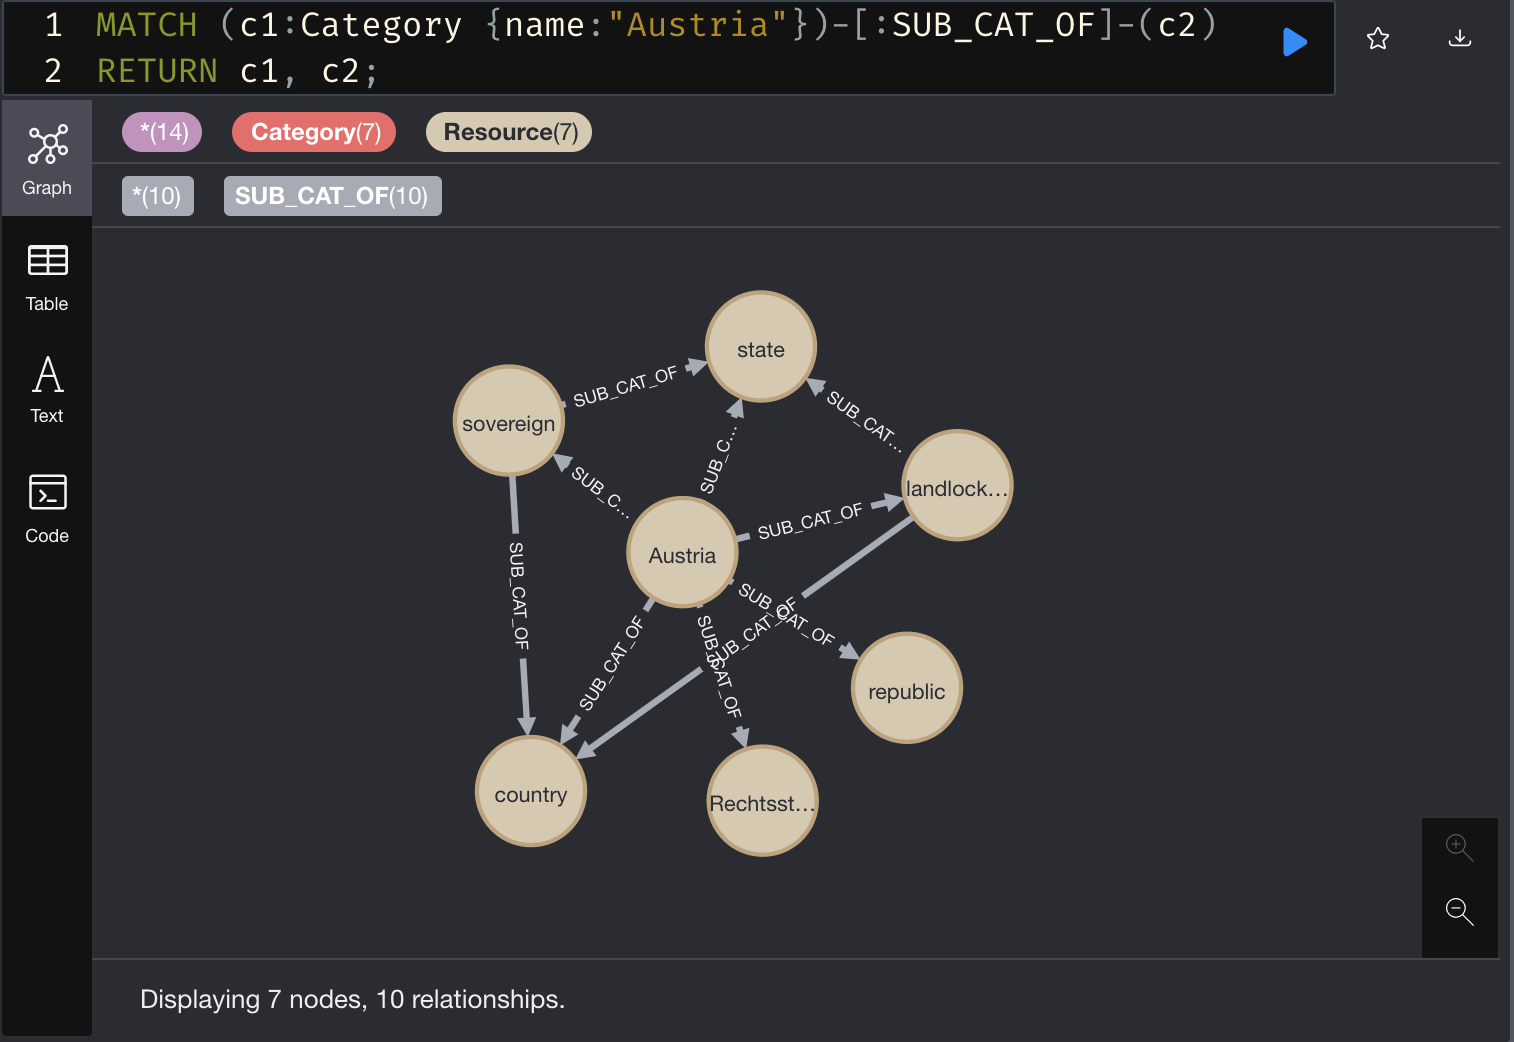
\includegraphics[scale=0.3]{use-case-1a}}

    From there, she may seek to draw links to other similar categories and learn that Senegal, Brazil, and Transnistria\footnote{A ``de facto unrecognized state in Eastern Europe that has declared independence from Moldova" (\url{https://www.wikidata.org/wiki/Q907112})}.
  
    \centerline{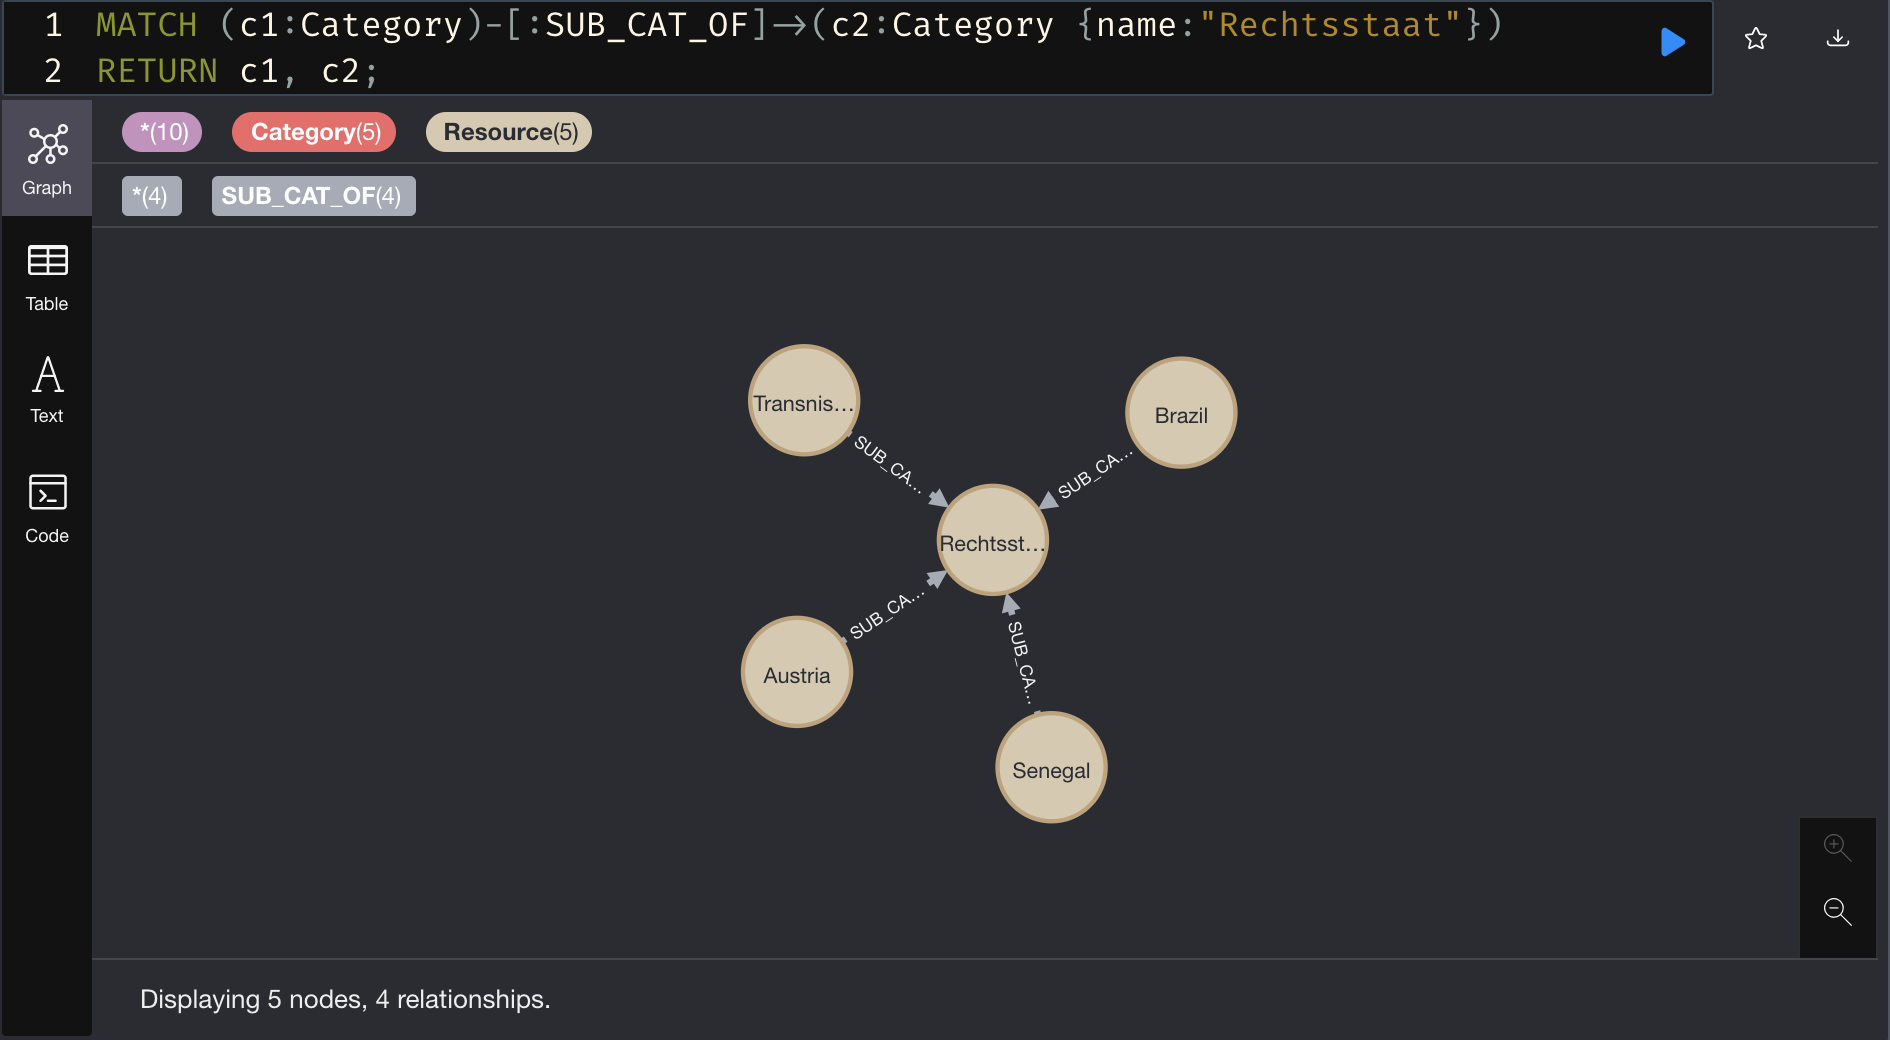
\includegraphics[scale=0.3]{use-case-1b}}

    Finally, she may be deepen her contextual knowledge by viewing any news items previously published about countries in a category like Rechtsstaat\footnote{A ``doctrine in European legal thinking, means `state based on justice and integrity'" (\url{https://www.wikidata.org/wiki/Q4209223})}.
  
    \centerline{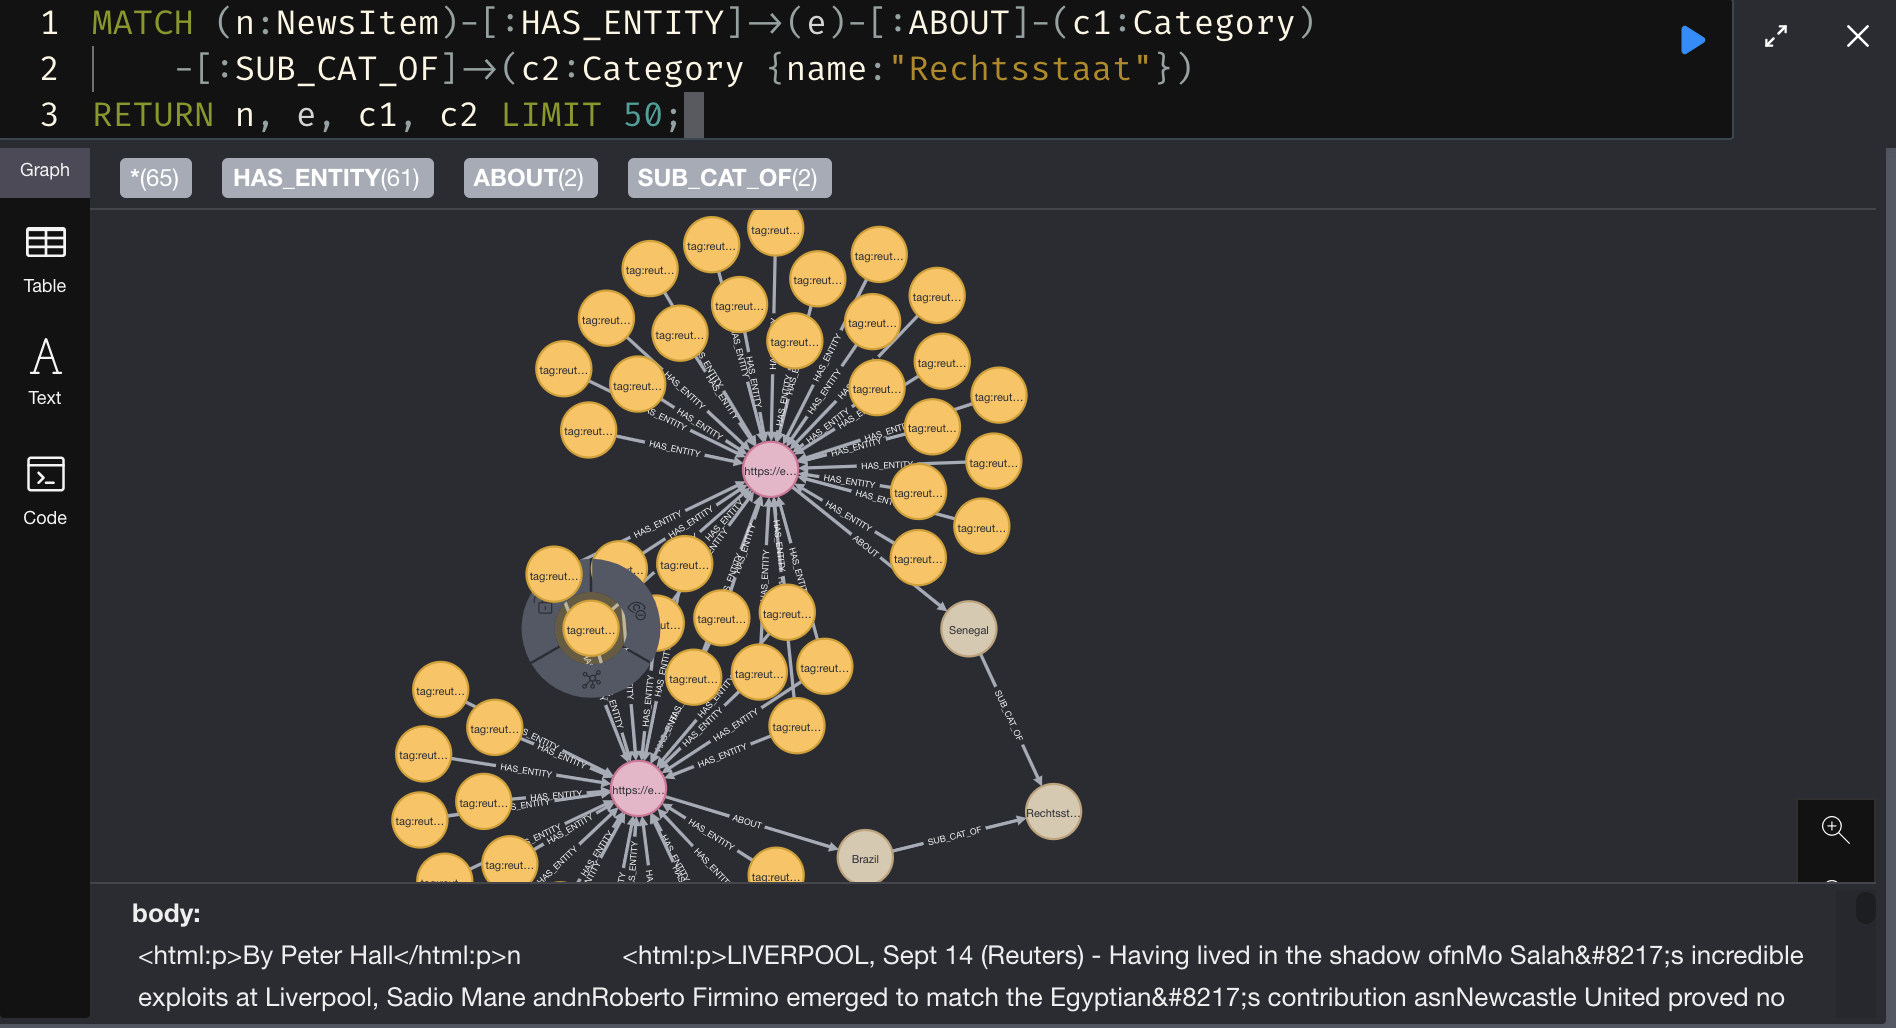
\includegraphics[scale=0.3]{use-case-1c}}
  }
  \item{
    \textit{Recommendations}: Media companies can leverage the knowledge graph as an API to provide recommendations to customers based on items they are viewing. This provides an improved user experience and increases the time the customers remain on the company's platform, thus increasing company revenue.

    For example, a customer may be reading a news article about football:

    \centerline{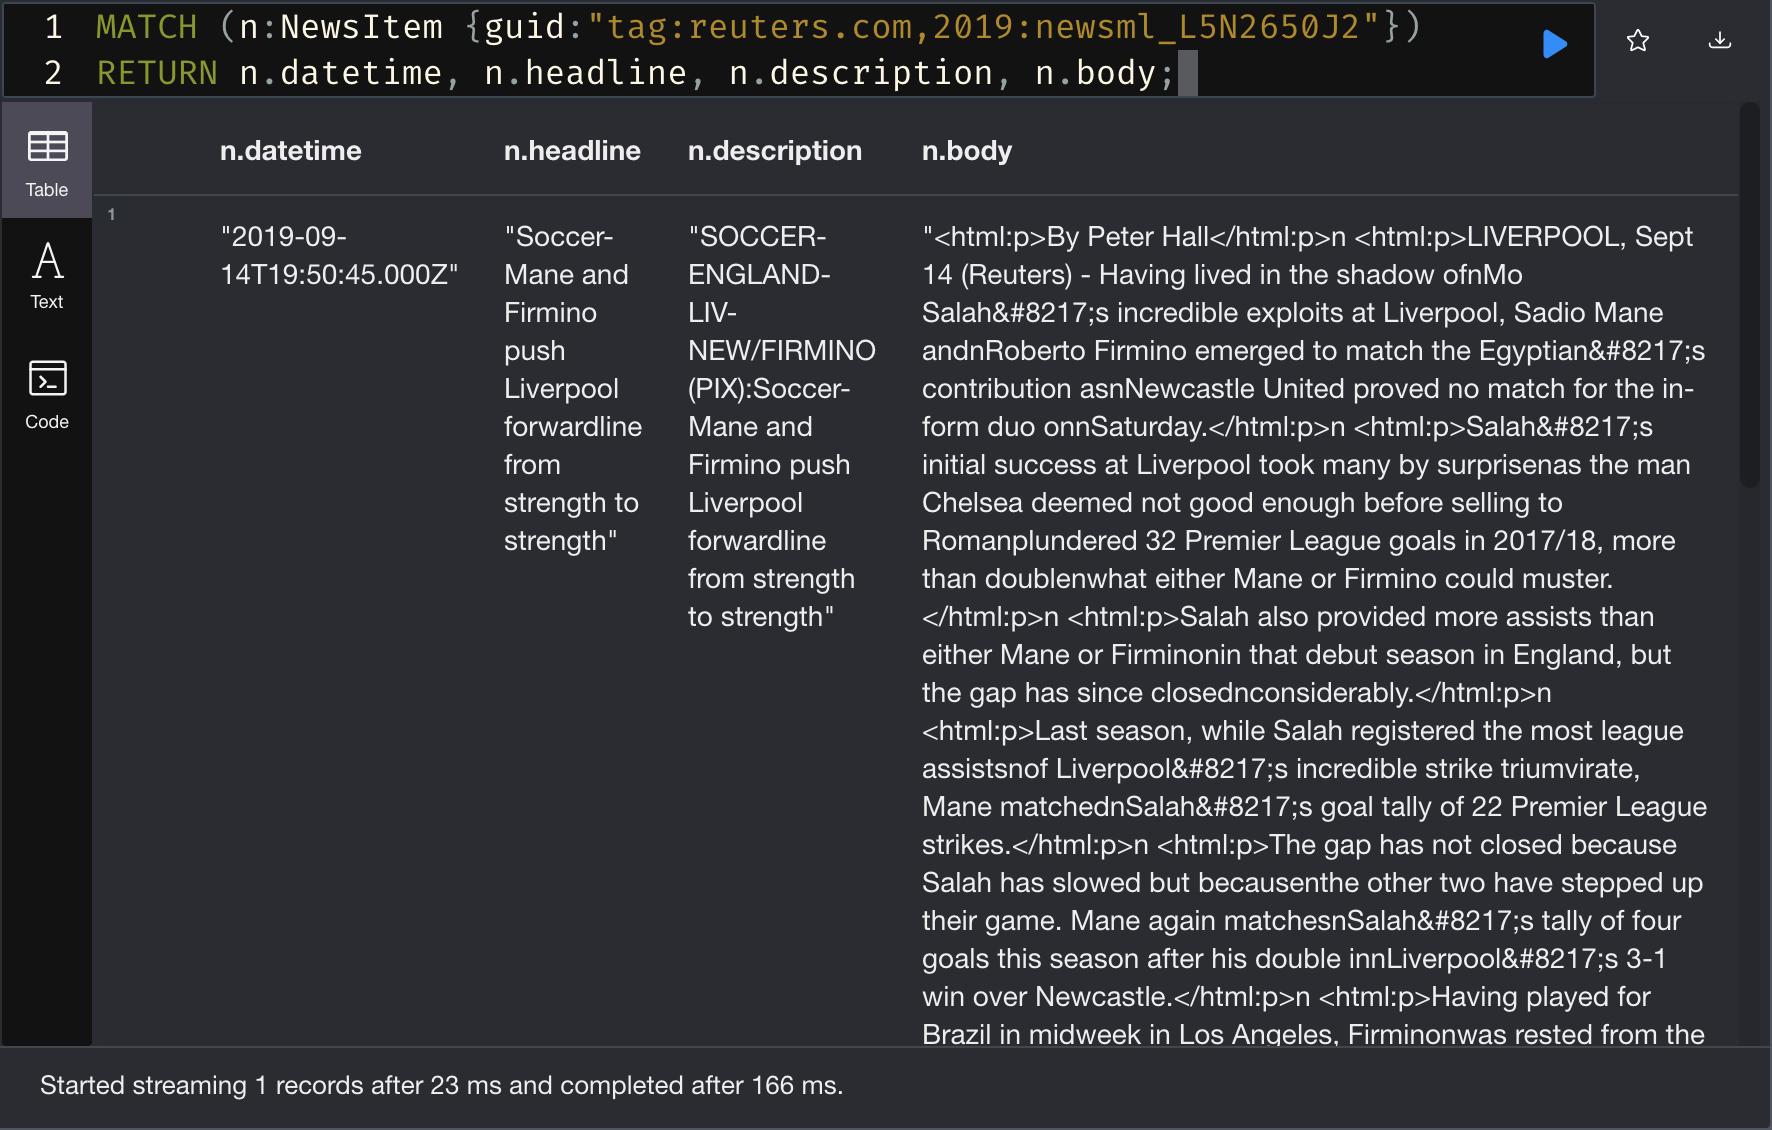
\includegraphics[scale=0.3]{use-case-2a}}

    The knowledge graph provides an easy way for the customer to view "similar" articles, by retrieving other articles that share knowledge graph paths to relevant football players:
    
    \centerline{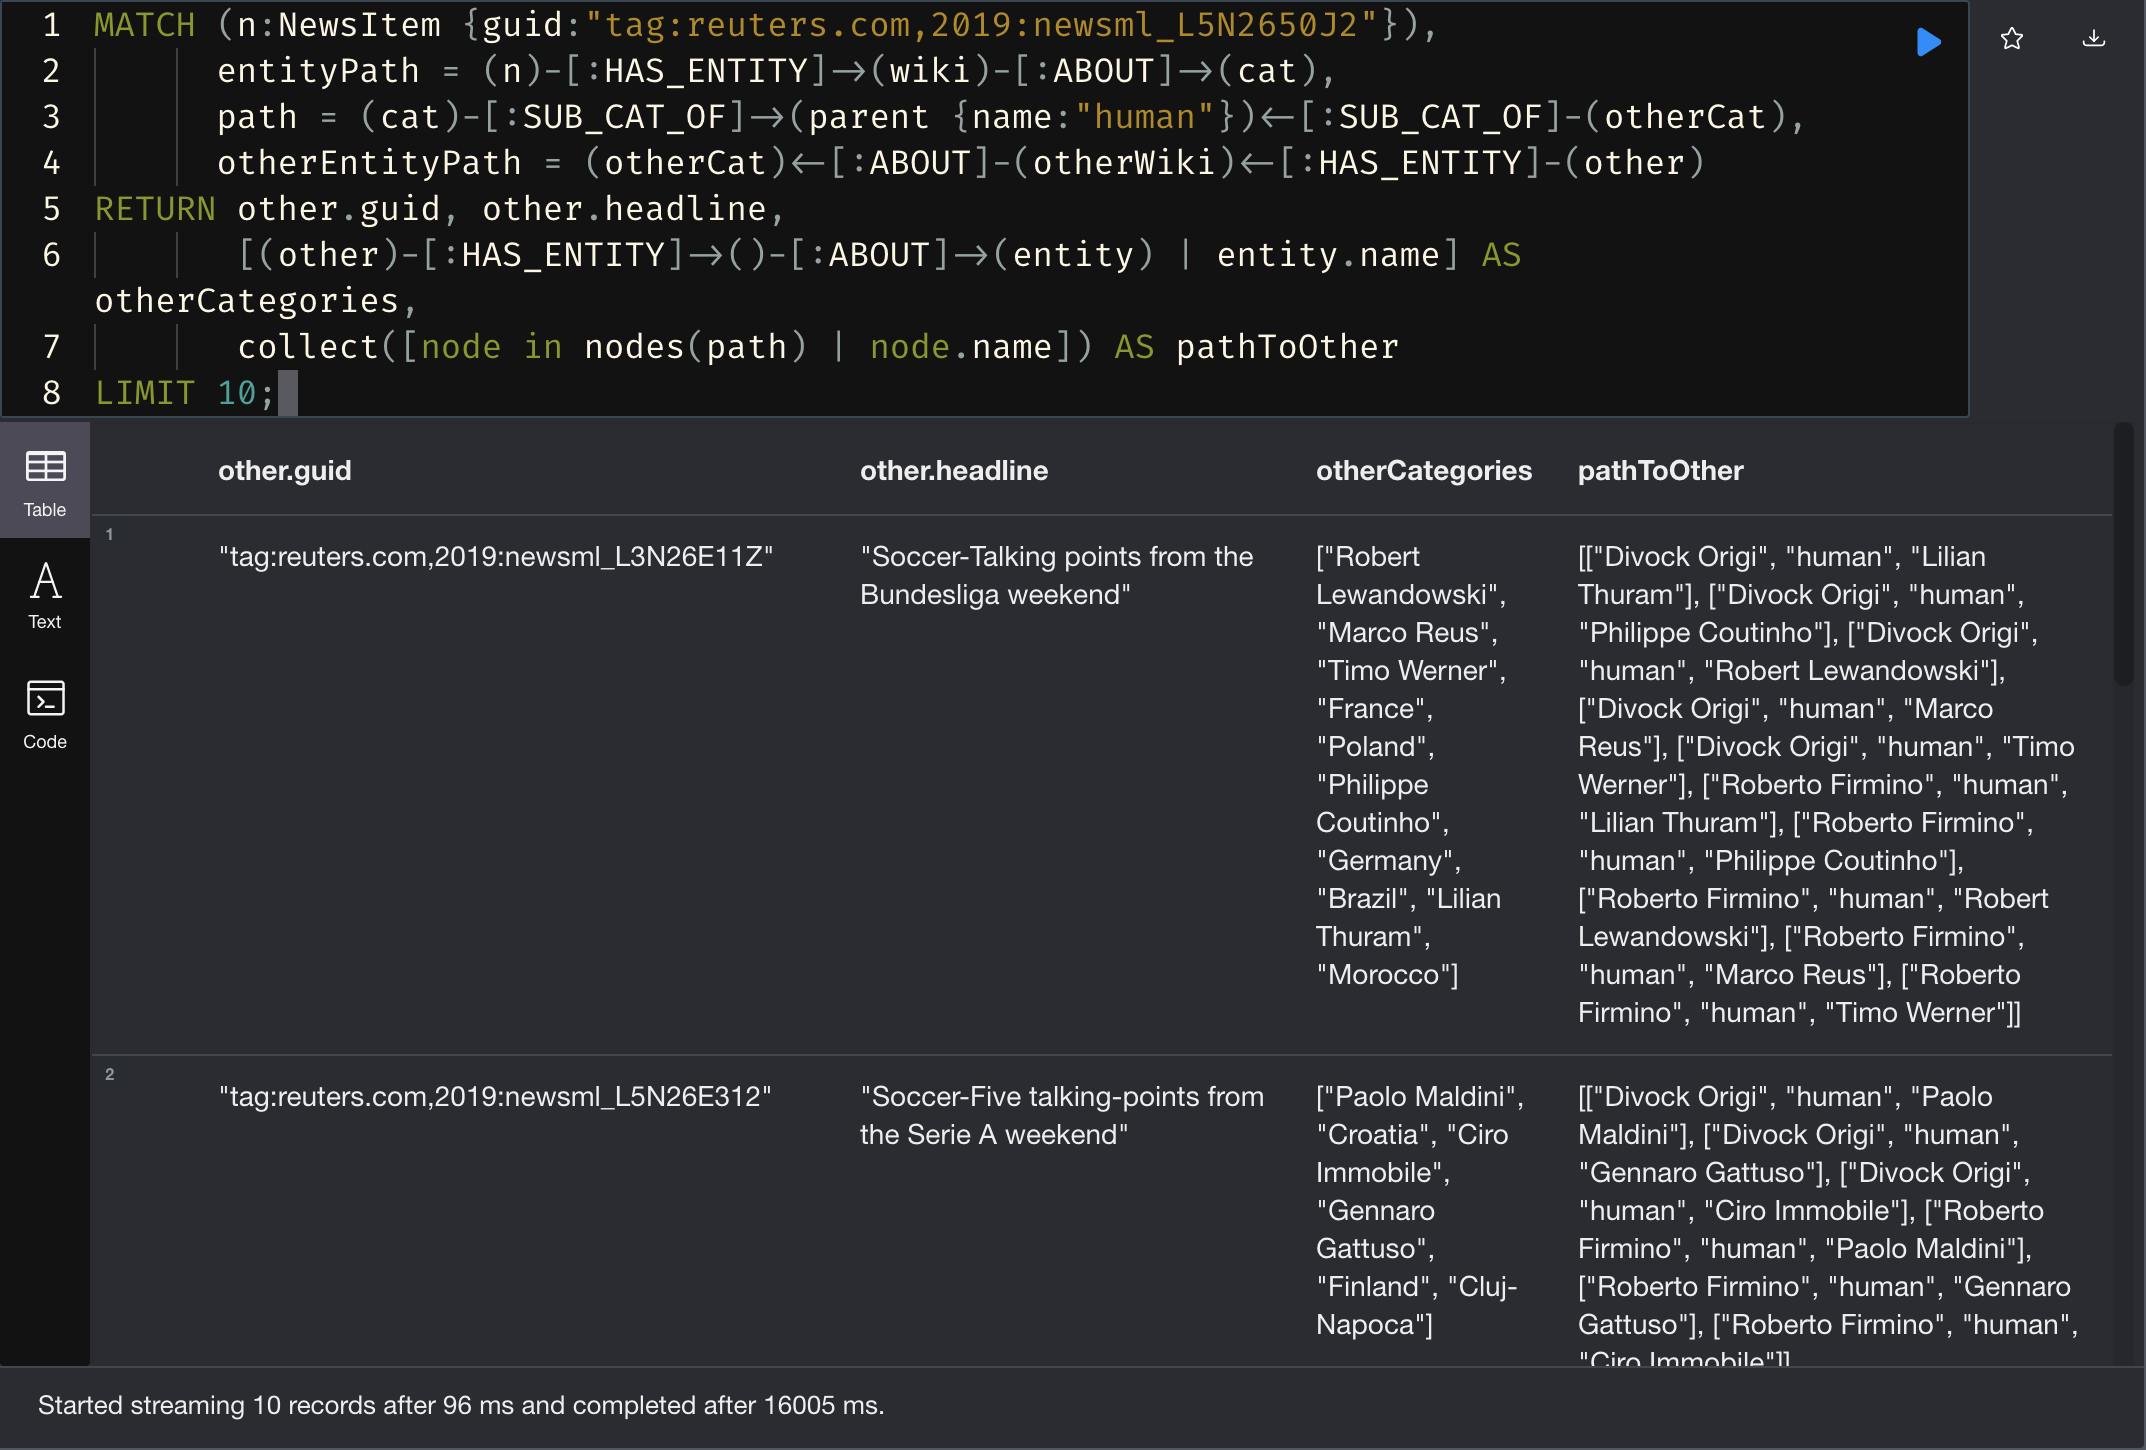
\includegraphics[scale=0.25]{use-case-2c}}
    }
\end{enumerate}

The second user type who would benefit from this pipeline and knowledge graph are \textbf{researchers and media customers}, who can use the knowledge graph for information retrieval and data mining. For example, the knowledge graph adds structure to semi-structured documents and draw meaning from the text in the following ways:
\begin{enumerate}
  \item{
    \textit{Entity extraction}: Entities have been extracted for each news item, enriching the news items' metadata and enabling users to identify the entities in a news item or news items about a given entity. A given news item's entities can be ranked based on their salience, giving an idea of each entity's relevance:

    \centerline{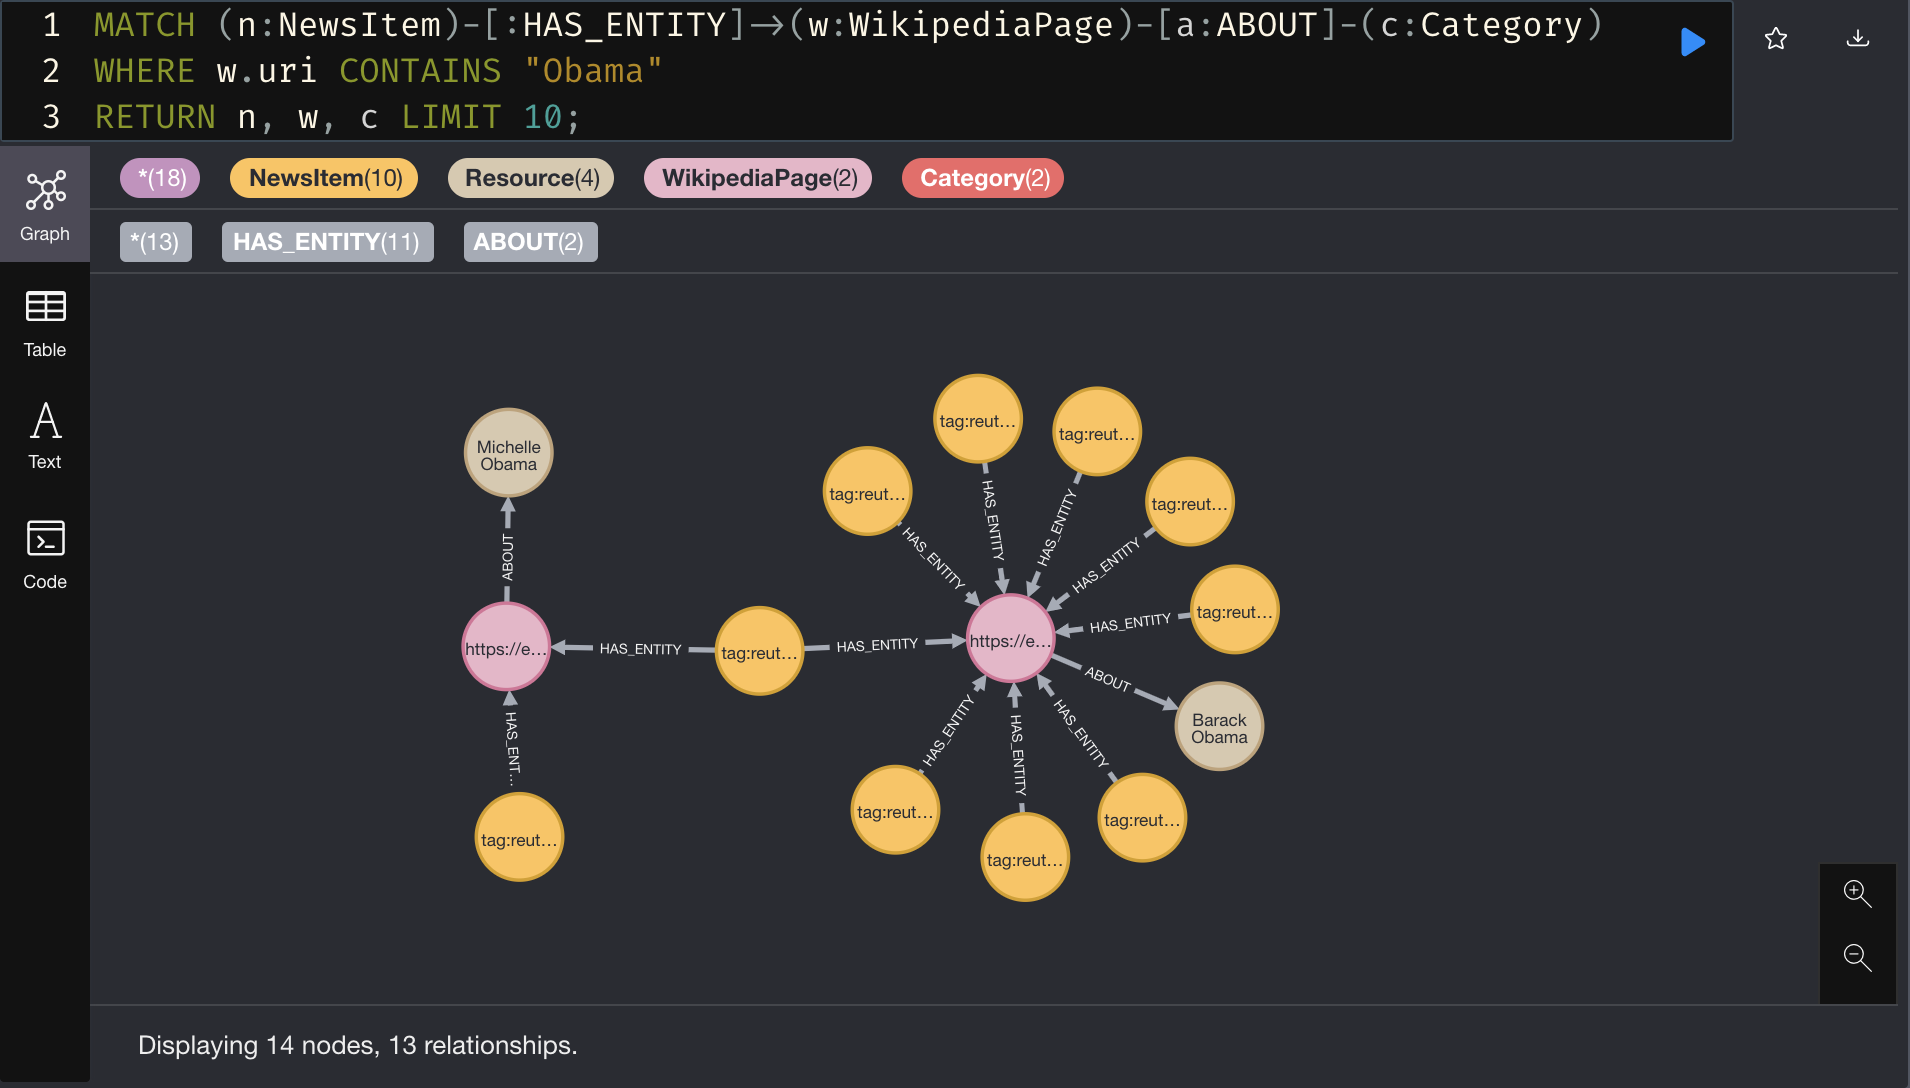
\includegraphics[scale=0.3]{use-case-3a}}
    \centerline{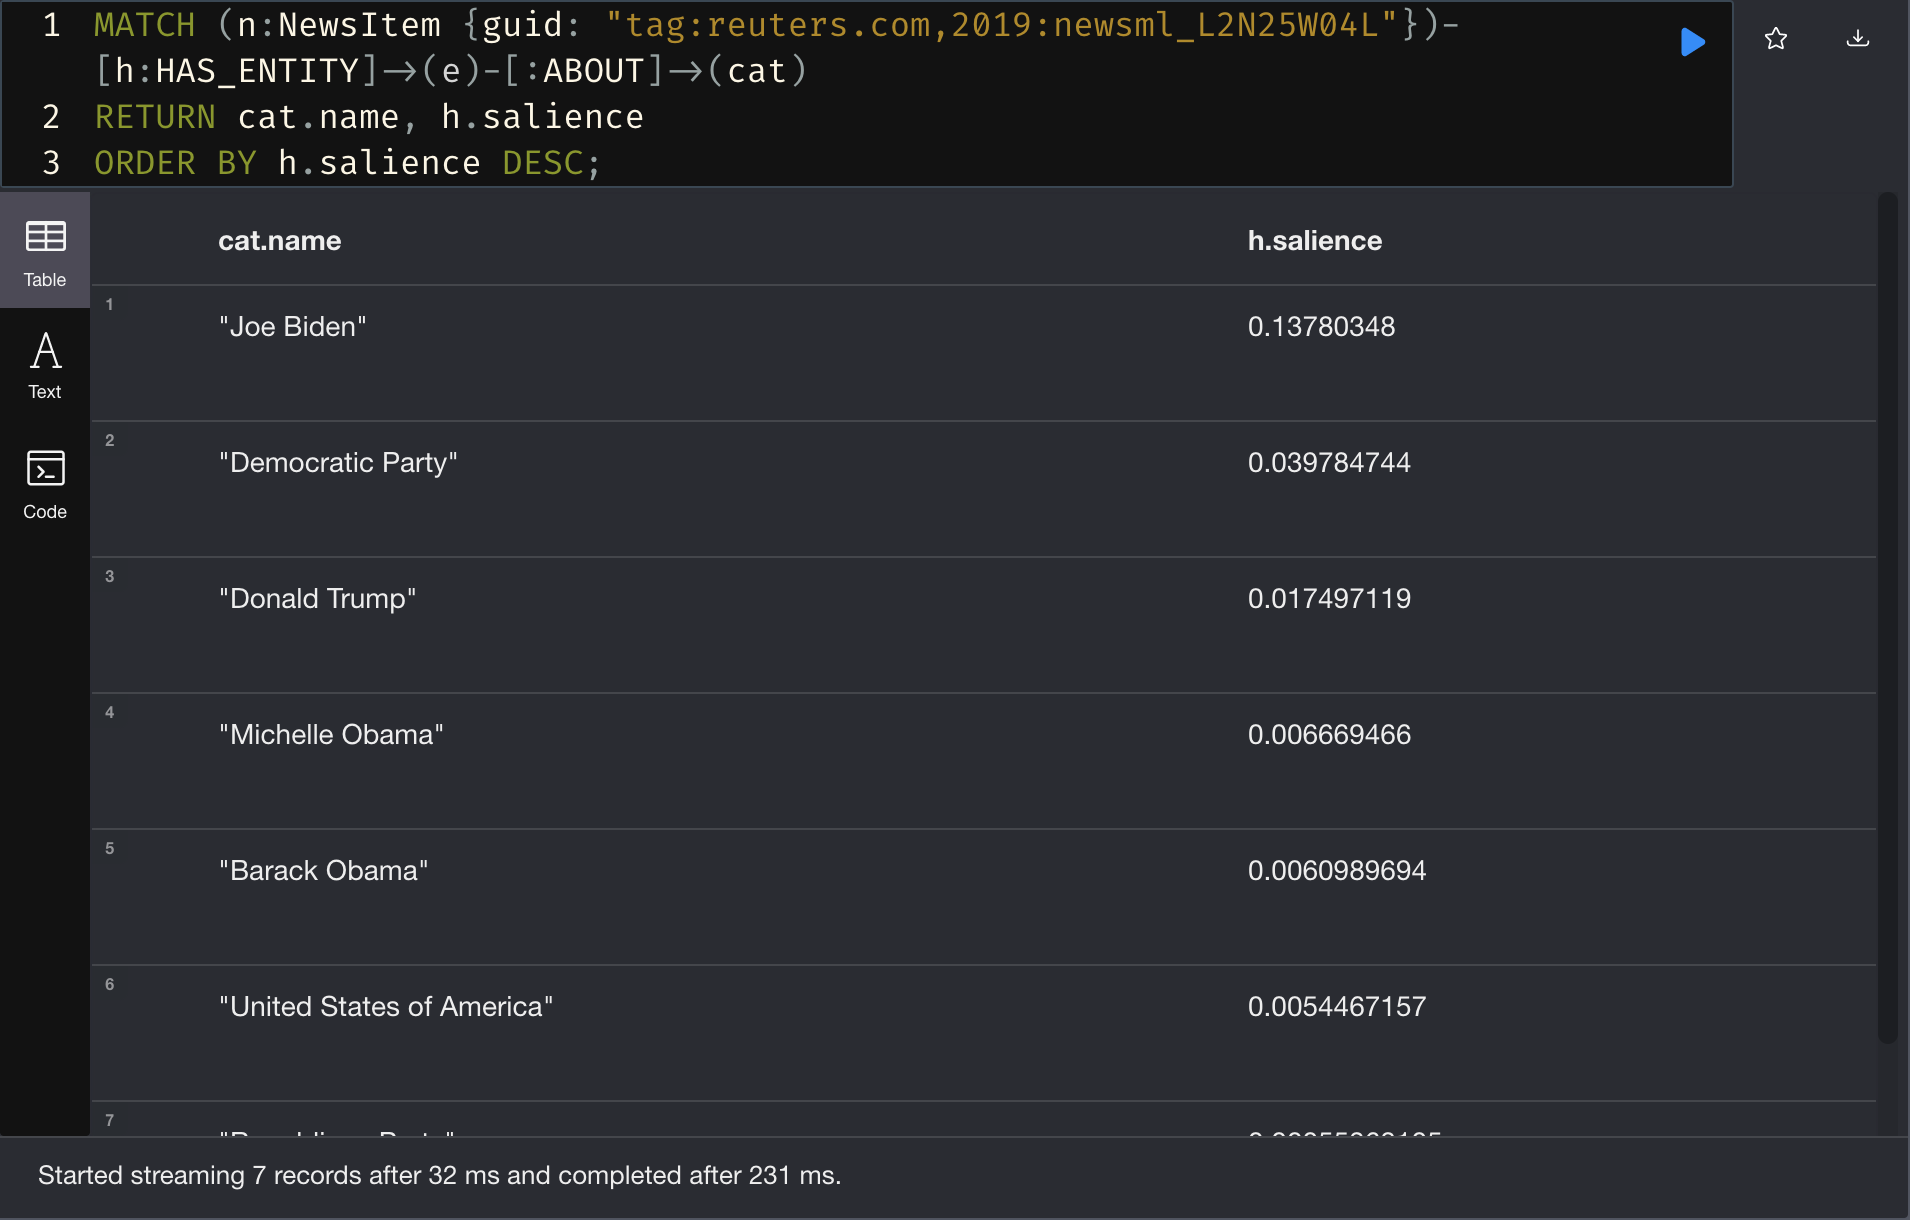
\includegraphics[scale=0.3]{use-case-3b}}

  }
  \item{
    \textit{Similarity}: News items can be similar based on shared relationships, as well as graph properties like K-nearest neighbours, Euclidean distance, or cosine similarity. As a simple example, Jaccard similarity can be computed using shared entities or subjects:

    \centerline{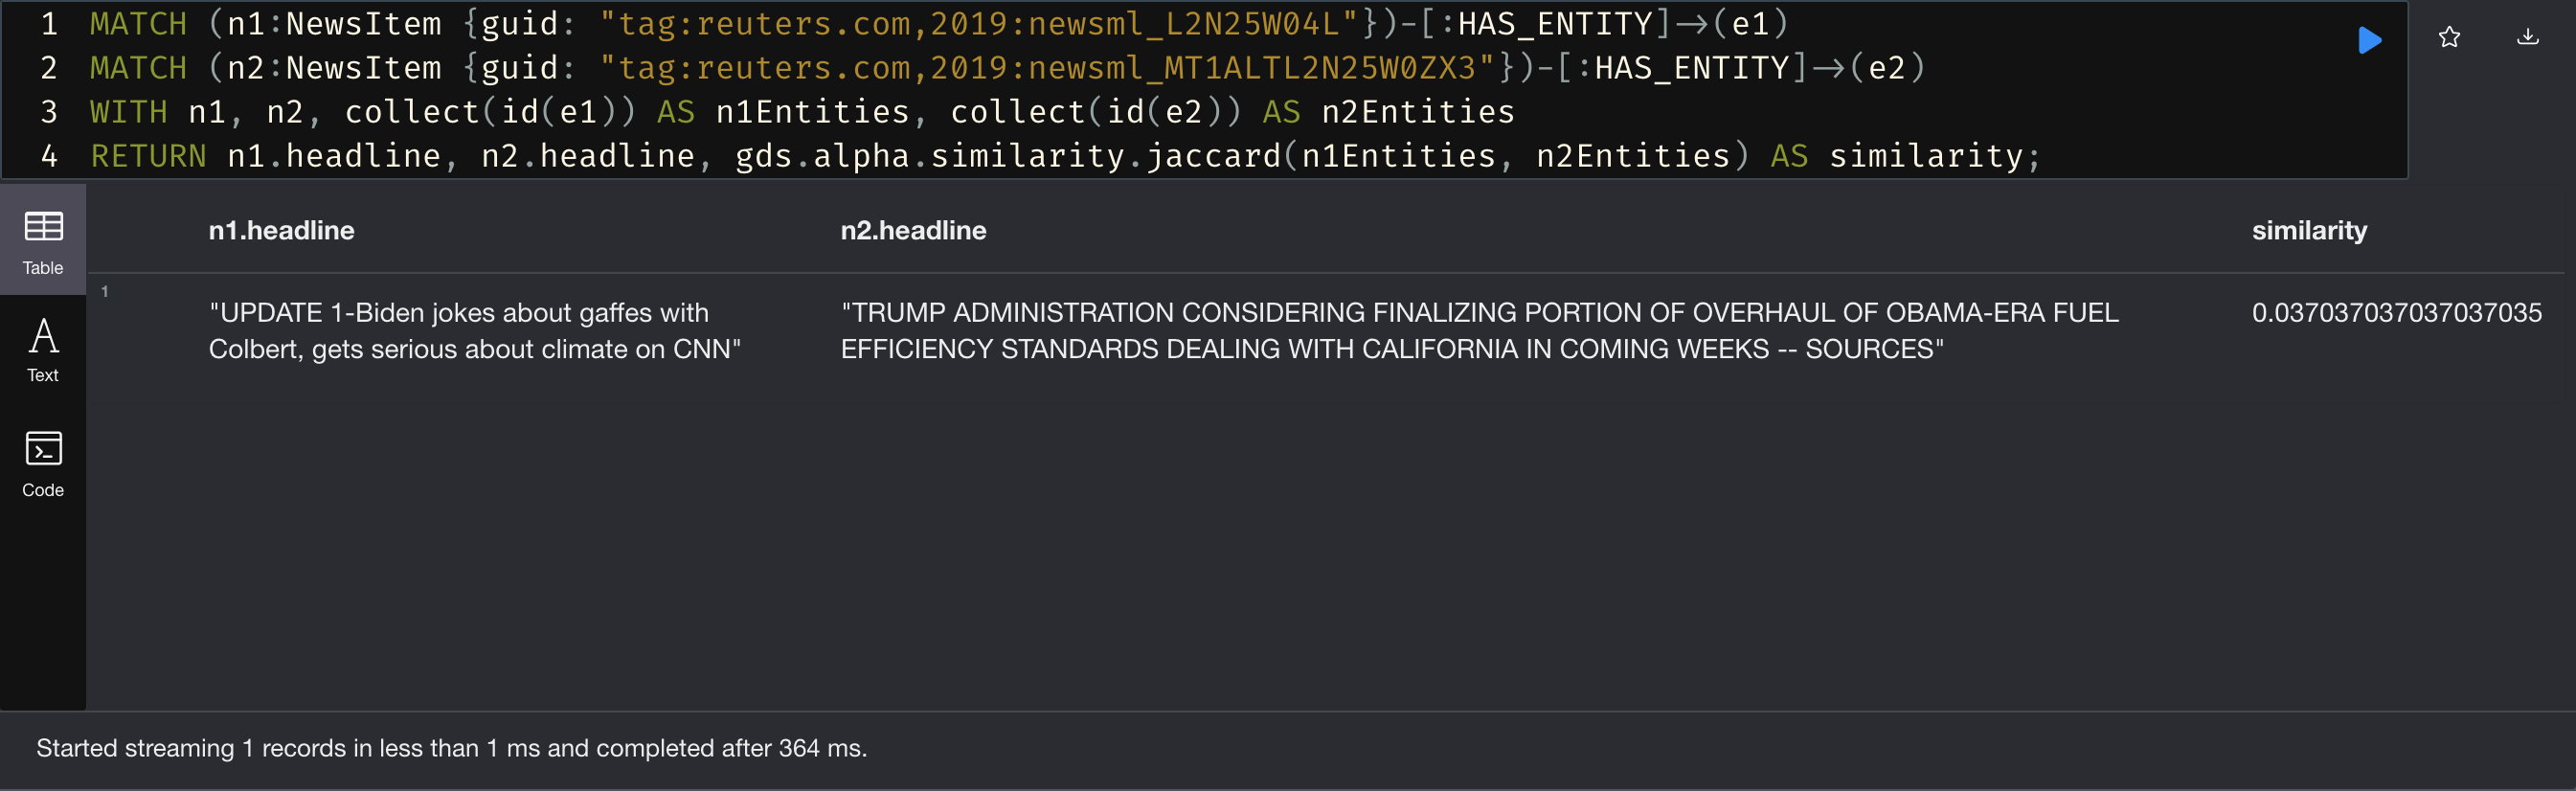
\includegraphics[scale=0.3]{use-case-4-similarity-1}}
  
    \centerline{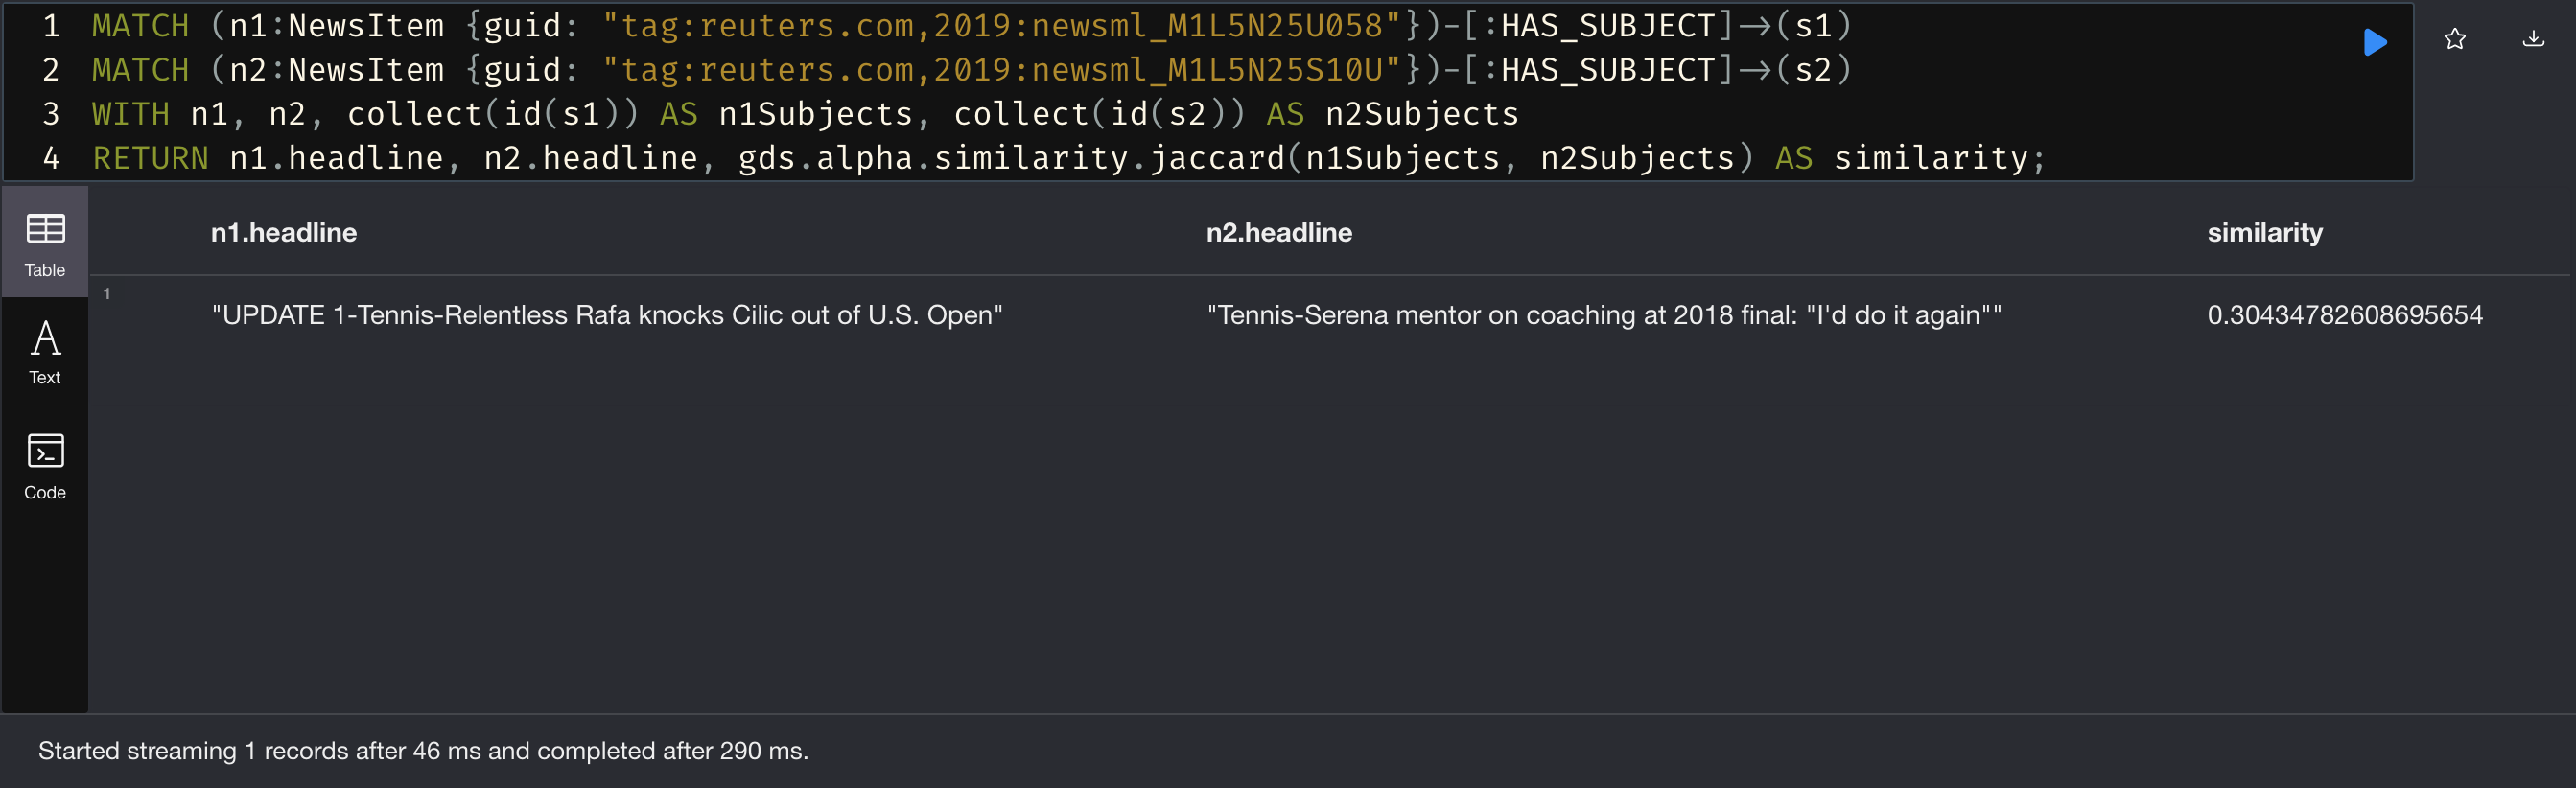
\includegraphics[scale=0.3]{use-case-4-similarity-2}}
  
    \centerline{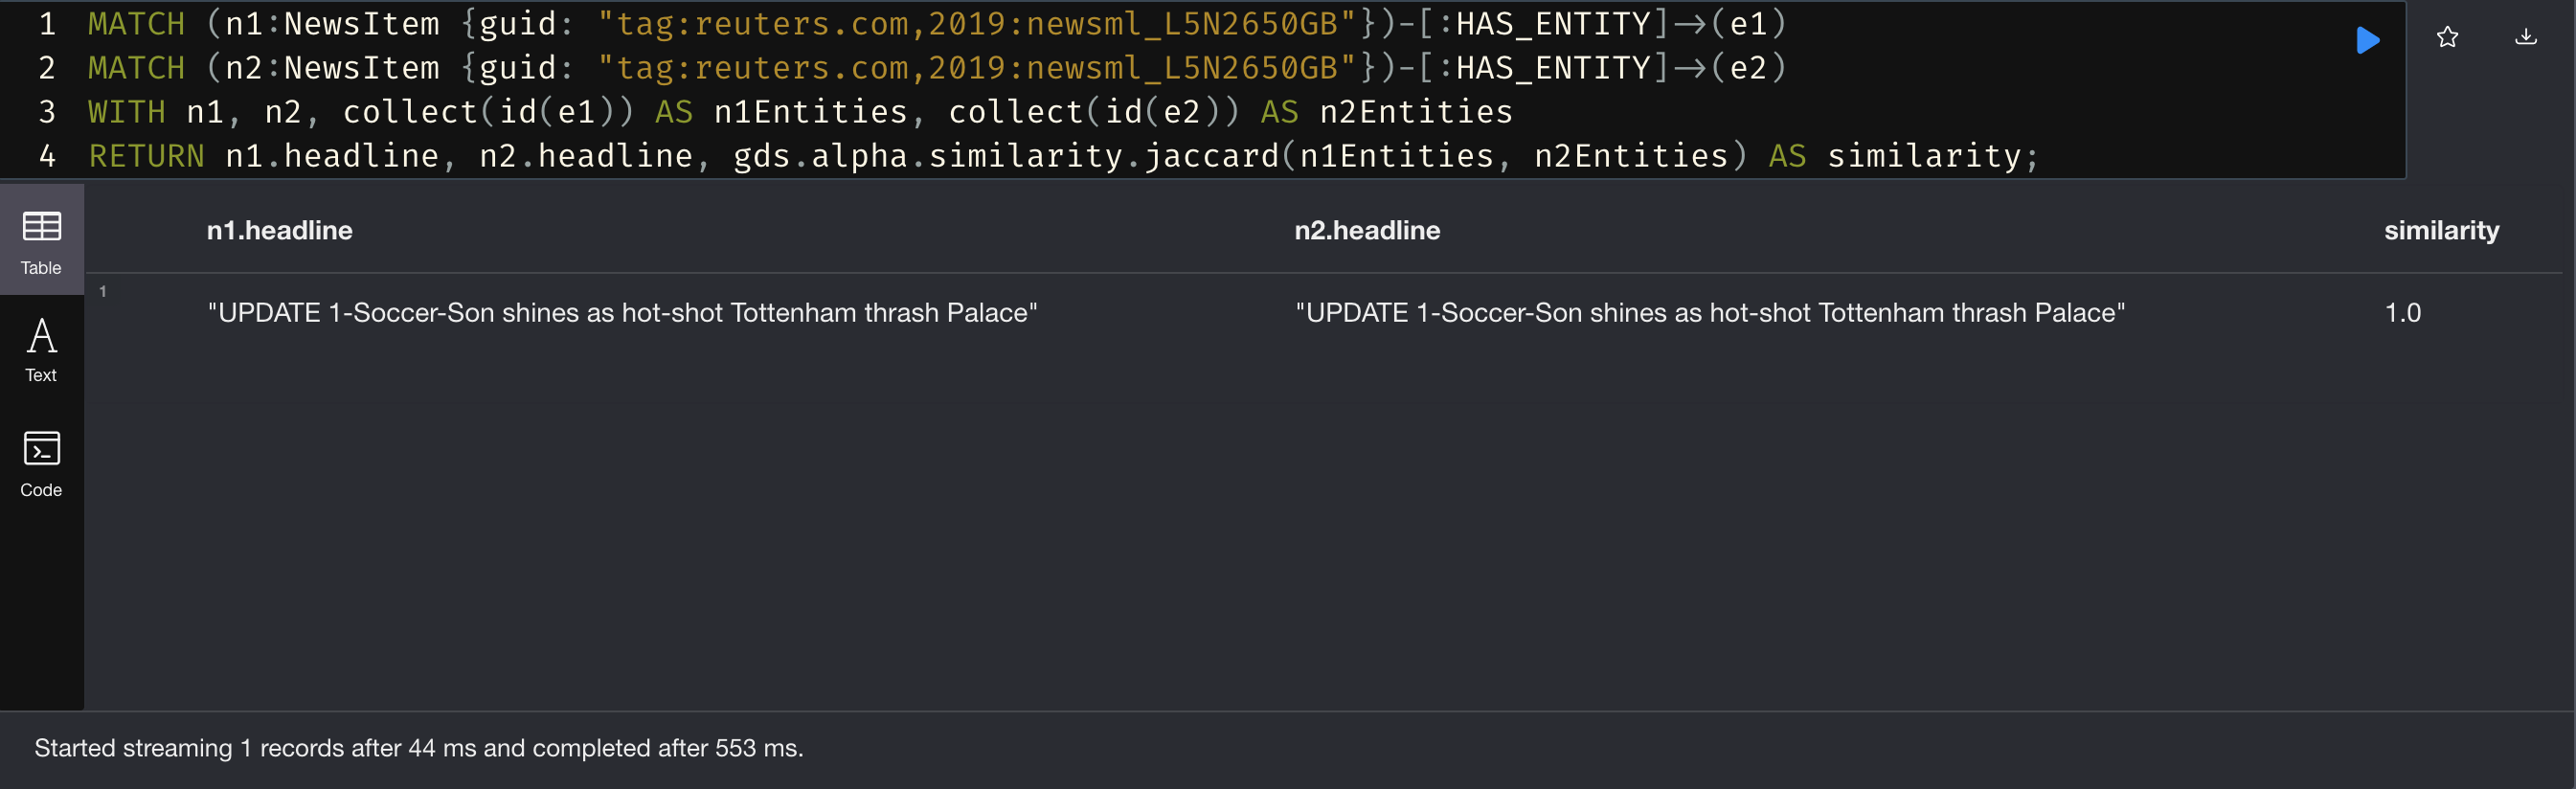
\includegraphics[scale=0.3]{use-case-4-similarity-3}}
  }
  \item{
    \textit{Categorisation}: By linking data with Wikidata, particularly Wikidata's ontology of categories and subcategories, the news items can be categorised in new ways. For example, categories enable unique queries like "all articles featuring landlocked countries" and provide additional details about companies like IBM as a public company, technology company, etc.:

    \centerline{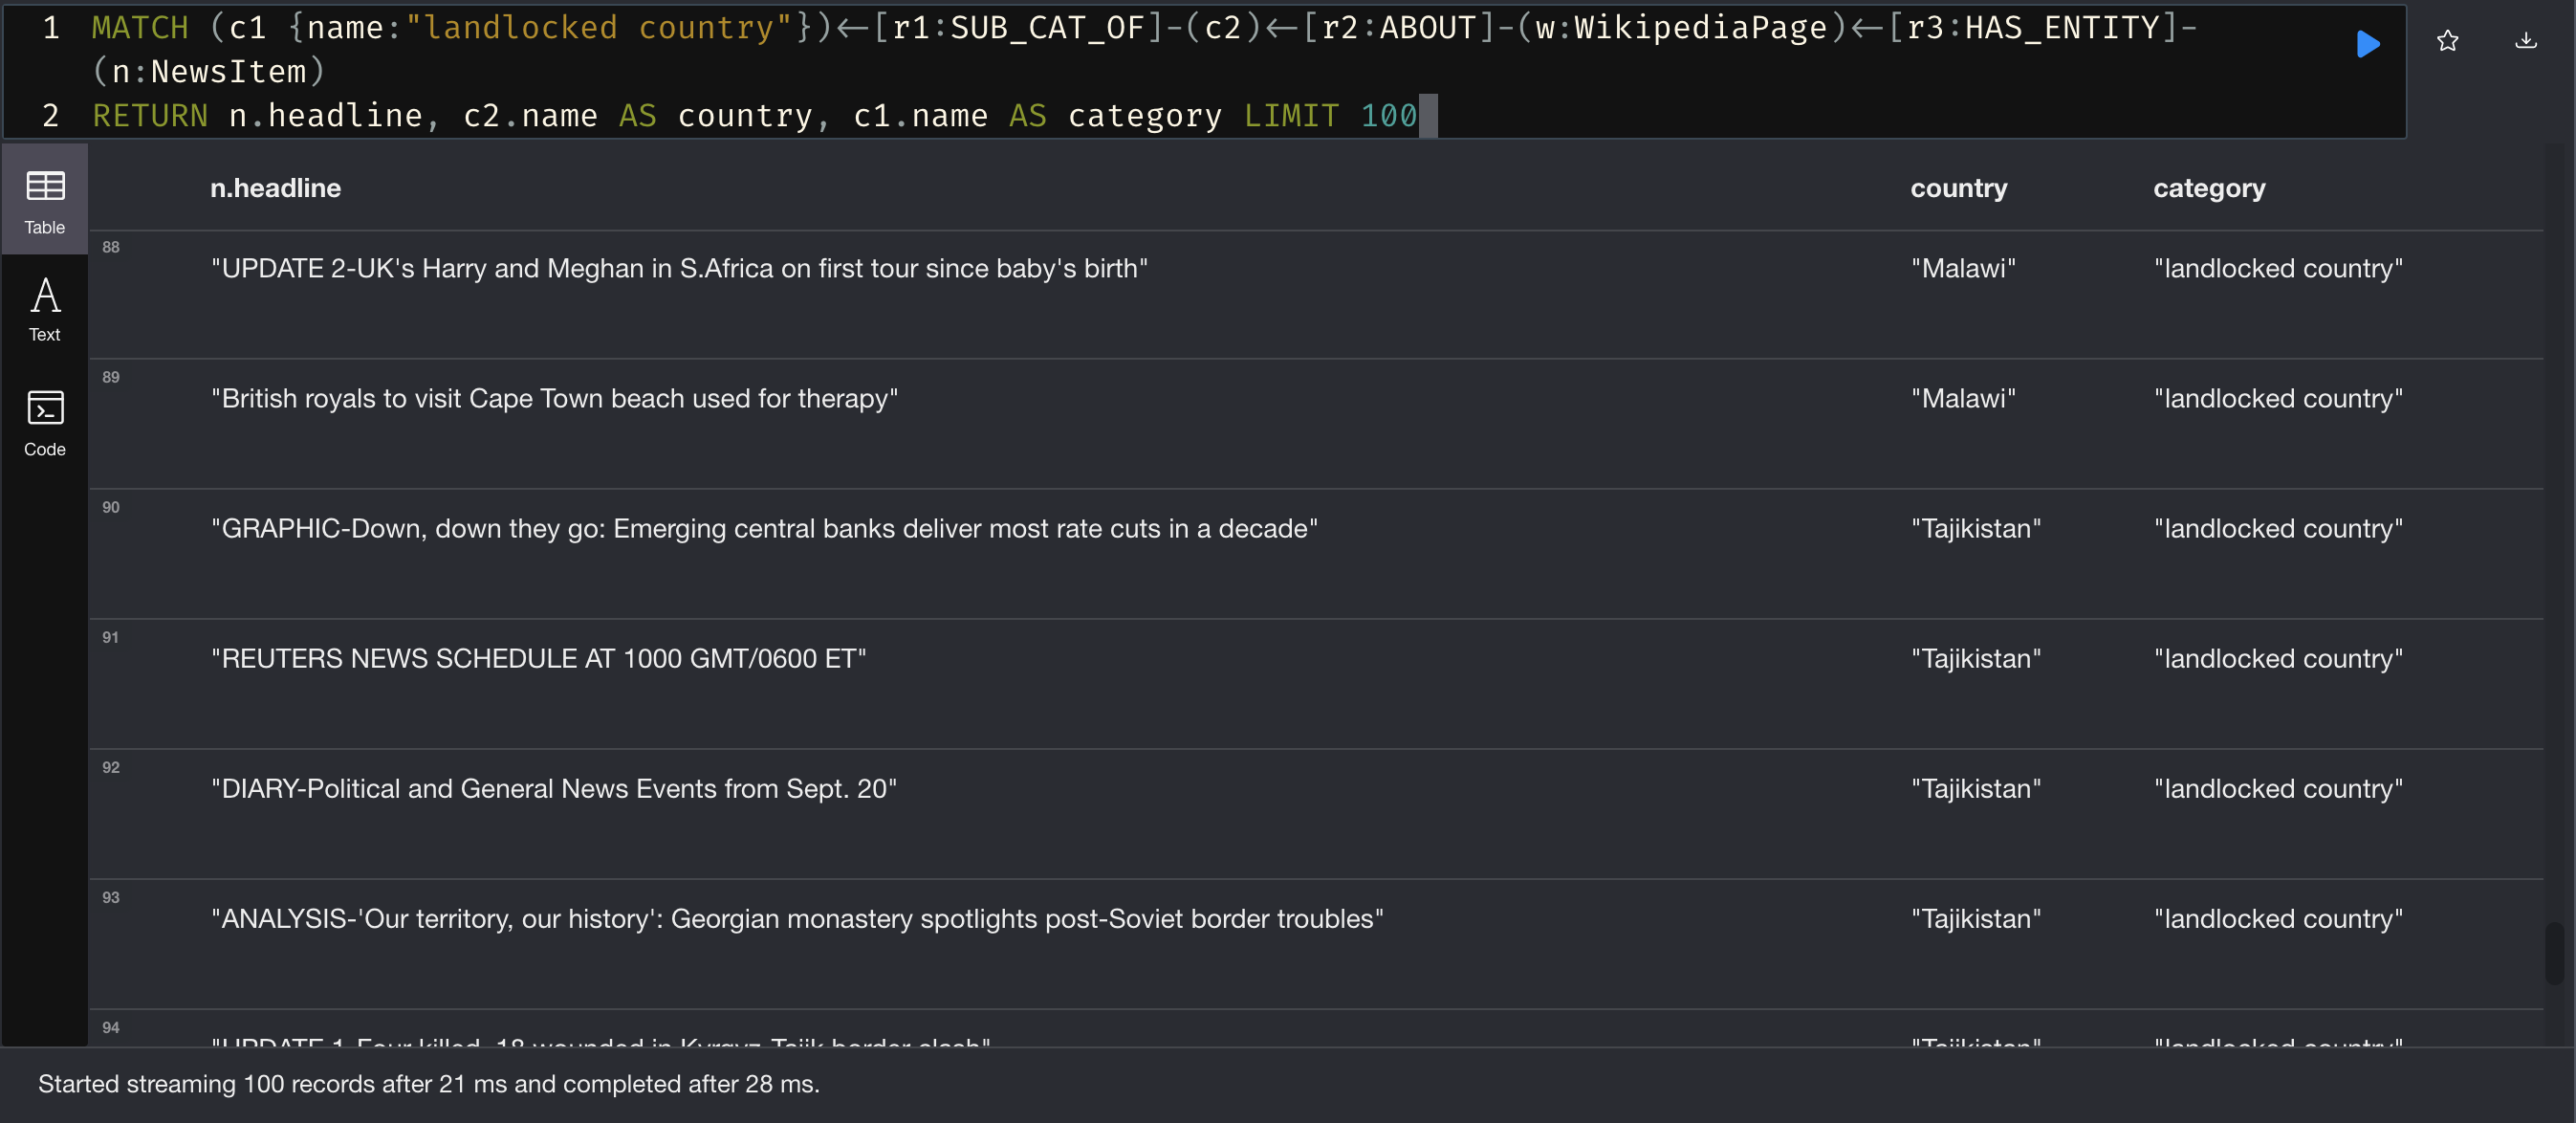
\includegraphics[scale=0.3]{use-case-5a}}

    \centerline{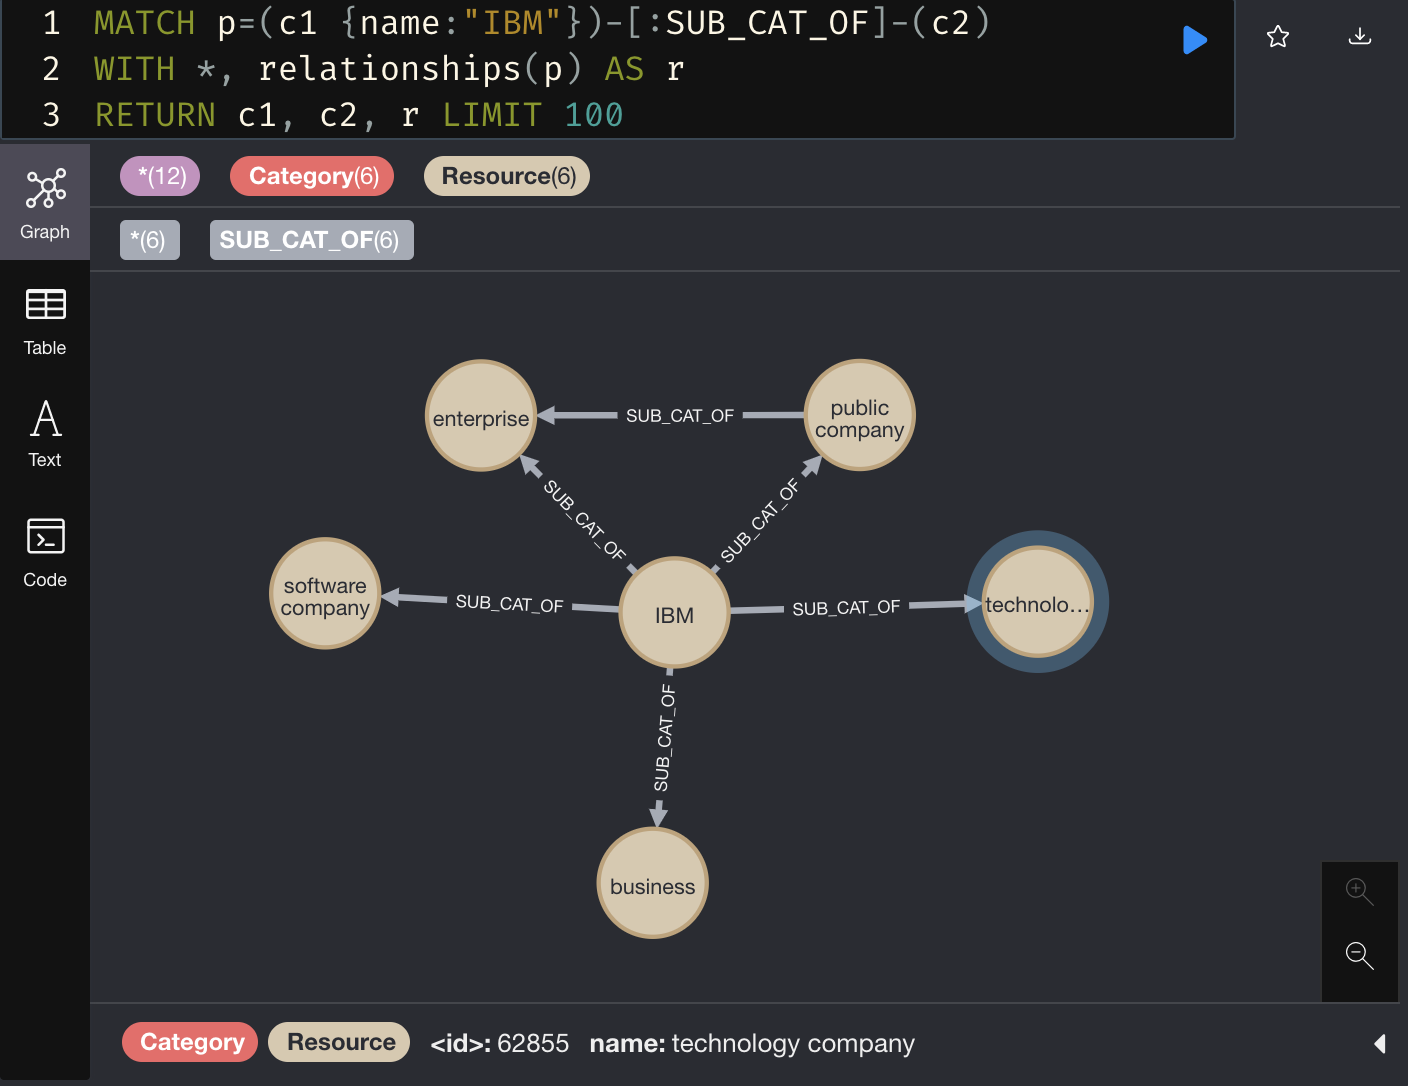
\includegraphics[scale=0.3]{use-case-5b}}
    }
\end{enumerate}
\subsection{Background}
The intent of this project is to build a knowledge graph for the news domain to improve news item recommendations and information retrieval. Knowledge graphs make use of the mathematical graph structure to enable knowledge representation or knowledge bases that can generate value in terms of human meaning.

News content is constantly generated by the media industry, providing a unique testing ground for knowledge graphs and their adjacent tehcnologies, due the the volume and structure of journalistic news. Published news items are rich in content and facts, but are generally unstructured and semantically limited, only accessible as free text. This presents information retrieval challenges for news consumers and an opportunity for a domain-specific knowledge graph architecture.

The report that follows will present a specification for a news knowledge graph, demonstrate an example data extraction pipeline, and present the final proof of concept knowledge graph system. Furthermore, it will experiment with related semantic technologies like ontologies and linked data and natural language processing (NLP) for entity extraction and link prediction. The final outcome is a working software and database system with value to the end user and as an example of a technical architecture for media practitioners.

\subsection{Aims and Objectives}
This project demonstrates the viability of a news information retrieval and recommendations system built with technologies including ontologies, linked data, and natural language processing. This proof of concept will be built using 59,542 items from the ``Reuters News Archive (30 Days)" dataset\footnote{\url{https://aws.amazon.com/marketplace/pp/prodview-qwmkdffmmjesa}}, to illustrate how informtation can be extracted from published news items and ingested into a knowledge graph. The end result is a knowledge graph which can be queried by an end user or can recommend a similar item of interest based on an item the user is reading.

As outlined in the project proposal\cite{ek-proposal}, the \textit{aims} include:
\begin{itemize}
  \item Design and implement a system for news information retrieval and recommendations
  \item Determine whether and how certain technologies, including knowledge graphs, ontologies, linked data, and natural language processing, can be used to implement such a system
\end{itemize}

The \textit{objectives} or concrete and verifiable outcomes include:
\begin{itemize}
  \item Develop a software specification for the design and implementation of an information retrieval system for news XML documents
  \item Build a data extraction pipeline for ingesting news data into the system
  \item Build a knowledge graph prototype stored in Neo4j and query-able via Cypher
  \item Experiment with semantic technologies and natural language processing for entity extraction and link prediction to enhance the knowledge graph
\end{itemize}

(Note to self: check back against proposal aims and objectives before finishing this section)
(Note to self: sections prefixed with "[WIP]" are "work in progress" as placeholders. This entire document is currently a work in progress and subject to change.)

\newpage
% \subsection{Problem}
% Problem...

% \subsection{Project Objectives}
% Project Objectives...

% \subsection{Summary of Findings}
% Summary of Findings...

% \subsection{Report Outline}
% Report Outline...

% \subsection{Technical Specifications}
% Technical Specifications...

% \section{Context and Background}
% TODO: repurpose some proposal sections...
% \subsection{Knowledge Graphs}
% \subsection{Network stuff?}
% similar to "A graph neural network path to network centralities.pdf"?
% % https://www.dcs.bbk.ac.uk/r/studentprojects/exampleprojects/msc/



\section{Literature Review}

\label{sec:LiteratureReview}

\subsection{News media knowledge graph literature}

As reviewed in the project proposal\cite{ek-proposal}, a number of knowledge representation systems have been proposed or built in the media industry as news-specific systems for the aggregation, generation, or linking of news articles. 

\begin{figure}
  \centerline{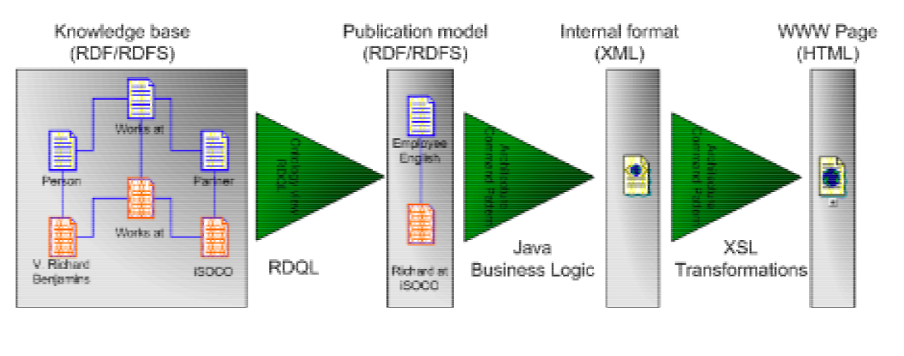
\includegraphics[scale=0.4]{literature-review--neptuno.png}}
  \caption{\textit{Neptuno diagram}}
\end{figure}

The first system of note historically is \textit{Neptuno} (2004)\cite{castells2004neptuno}, which introduces ``emergent semantic-based technologies to improve the processes of creation, maintenance, and exploitation of the digital archive of a newspaper". This archive-focused technique presents useful background for this project, but is oriented as an ontology-first approach. For example, Neptuno's ``Publication through visualisation ontology" model begins with RDF and ends with XML and HTML, whereas this project begins with published XML documents (see "Figure 1").

\begin{figure}
  \centerline{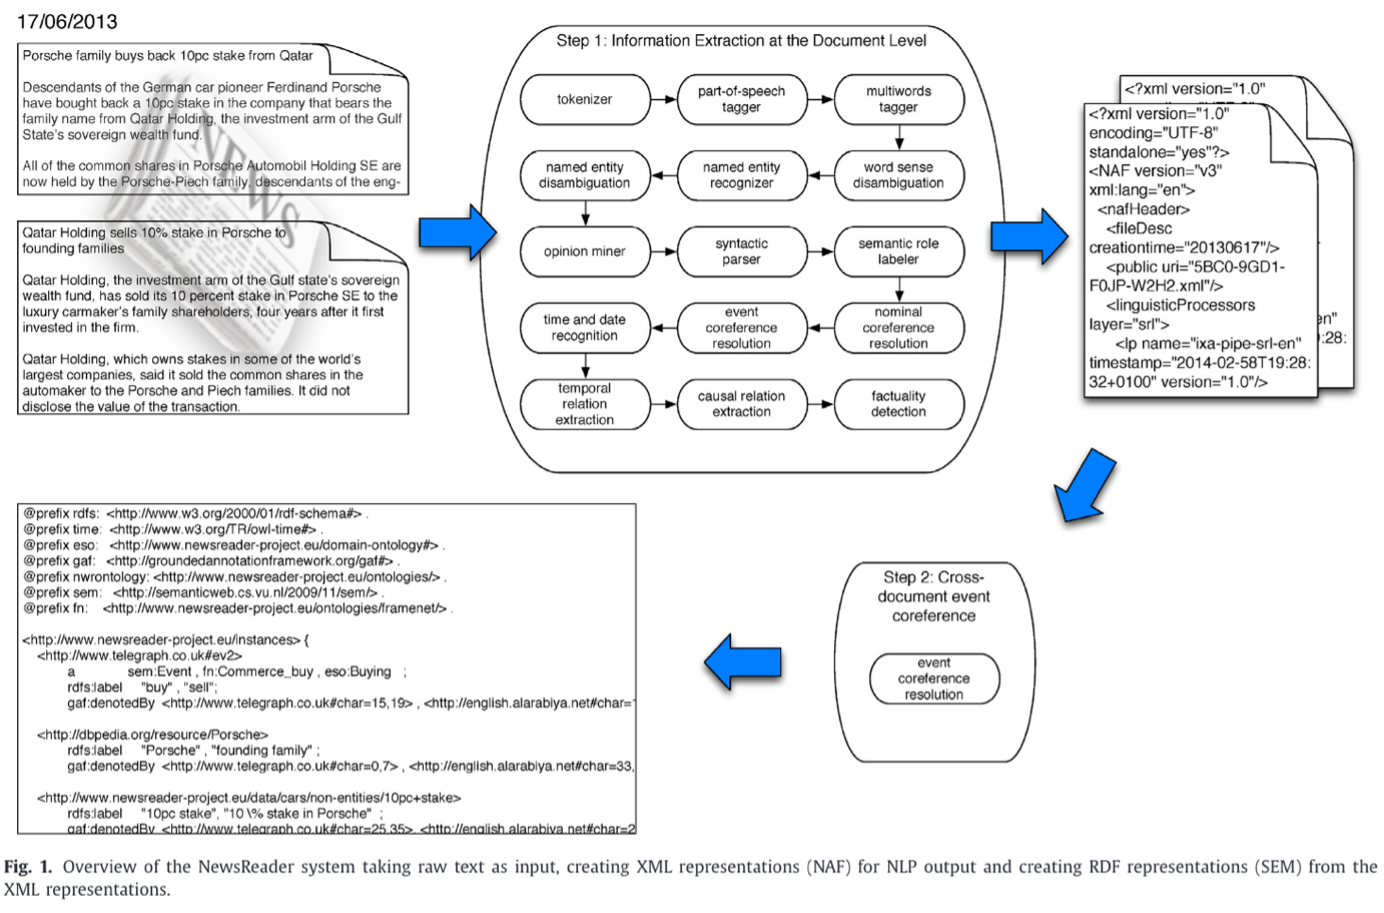
\includegraphics[scale=0.4]{literature-review--newsreader.png}}
  \caption{\textit{NewsReader diagram}}
\end{figure}

Meanwhile, \textit{News Engine Web Services (NEWS)} \cite{fernandez2010news} (2010), \textit{NewsReader} \cite{vossen2016newsreader} (2016), and \textit{Acquisition de Schémas pour la Reconnaissance et l'Annotation d'Événements Liés (ASRAEL)} \cite{rudnik2019searching} (2019) each approach the news industry from a semantic technology point of view, using ontology, metadata vocabularies, RDF, and Wikidata. NewsReader, for example, matches the sequence of operations that this project proposes, from raw text to information extraction, linked data, and ontology development (see "Figure 2").

\begin{figure}
  \centerline{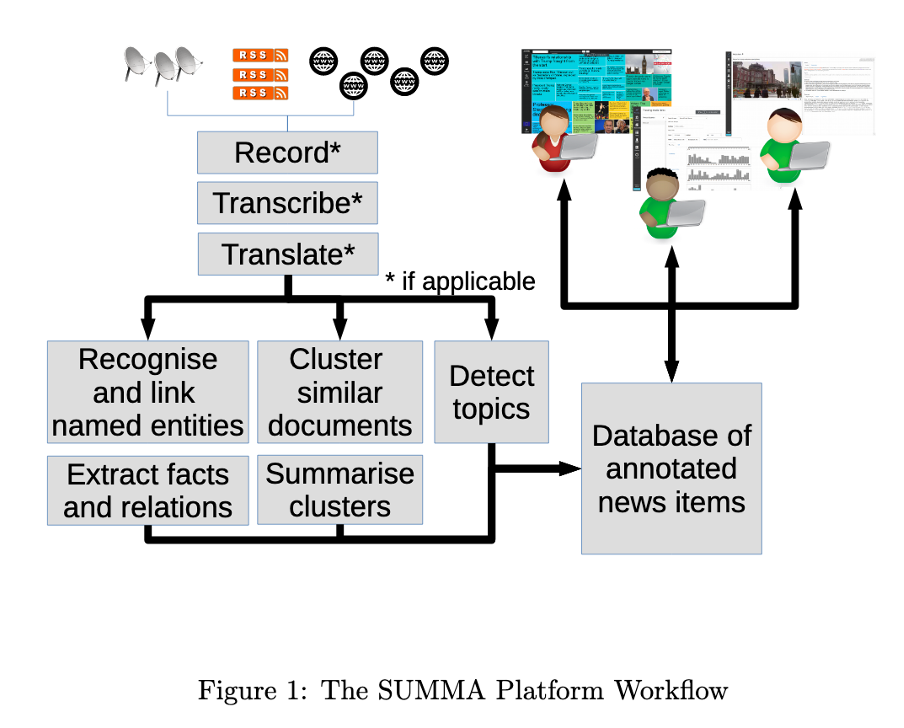
\includegraphics[scale=0.4]{literature-review--summa.png}}
  \caption{\textit{SUMMA diagram}}
\end{figure}

Two recent efforts have applied NLP and ML techniques to news data. These are \textit{Scalable Understanding of Multilingual MediA (SUMMA)} \cite{germann2018integrating} (2018) and \textit{News Hunter} \cite{berven2020knowledge} (2020), which are both platforms and architectures for news monitoring and applying NLP pipelines. For example, SUMMA matches the general data flow proposed in this project (see "Figure 3"). Furthermore, it presents useful state of the art for NLP techniques, including entity extraction, clustering, and topic detection, which will be pursued in this project.

\begin{figure}
  \centerline{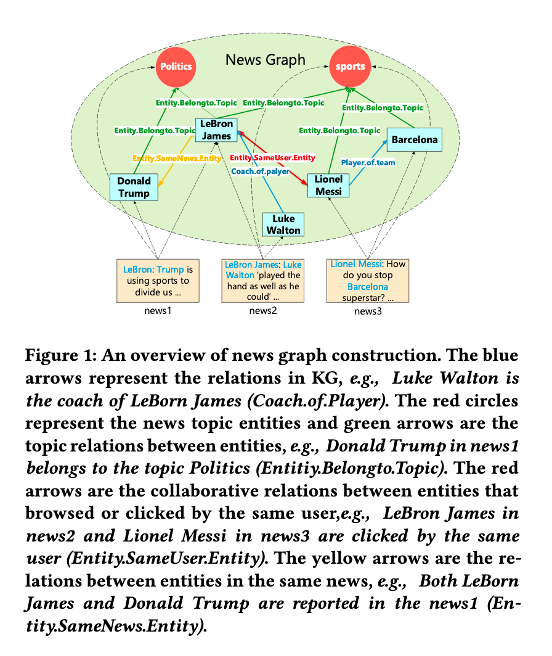
\includegraphics[scale=0.4]{literature-review--newsgraph.png}}
  \caption{\textit{SUMMA diagram}}
\end{figure}

\textit{News Graph} \cite{liu2019news} (2019), may be the research most directly relevant to this project. As an enhanced news knowledge graph that adds new entities and relationships and removes news-irrelevant links, it models the desired outcome of news recommendations based on the application of NLP techniques. On the other hand, it focuses on mathematical techniques around entity embeddings for news recommendations; this is of note for the project, but goes deeply into a specific direction rather than as a general knowledge graph in the news domain.

Finally, a number of other systems were reviewed, but deemed not relevant to the project at hand. These include \textit{Global Database of Events, Language, and Tone (GDELT)}\footnote{\url{https://www.gdeltproject.org/}} (2013) and \textit{Event Registry} \cite{leban2014event} (2014), which were proposed as real-time monitoring systems for analysing "world events" or "world's news media". These both approach the field differently, as a high-volume monitoring system rather than a knowledge graph architecture for information retrieval. Furthermore, \textit{NewsAPI}\footnote{\url{https://newsapi.org/}} (2017) is JSON API to retrieve articles and breaking news headlines from various sources, but not an overall knowledge architecture. Finally, \textit{Reuters' Tracer} \cite{liu2017reuters} (2017) ``automates end-to-end news production using Twitter data." It provides an interesting example of a data pipeline, but with a different use case.

\subsection{Knowledge Graph literature}

In addition to the literature on news-specific knowledge systems, there is a wealth of resources related to knowledge graph architecture more broadly. For example, \textit{Architecture of knowledge graph construction techniques} (2018) \cite{zhao2018architecture} presents a helpful distinction between two types of knowledge graph approaches:

\begin{displayquote}
In the top-down approach emphasizing the well-defined domain ontologies, the domain ontologies and their schema should be defined at first, and then [...] knowledge instances are added into knowledge base. The bottom-up approach extracts knowledge instances from knowledge resources. After knowledge fusing the populated instances, the top-level ontologies are built by means of knowledge instances to create the whole KGs.
\end{displayquote}

This clarifies that the news domain knowledge graph proposed in this project takes a bottom-up approach, starting from the text data and building up to entity extraction and ontologies.

Two other useful resources are \textit{A review of relational machine learning for knowledge graphs} \cite{nickel2015review} and \textit{Knowledge graph embedding: A survey of approaches and applications} \cite{wang2017knowledge}, which review the application of relational machine learning and graph embedding in the knowledge graph domain. These techniques are out of scope for this effort, but present interesting opportunities for future research.

\section{Data Extraction and Software Specification}
\subsection{Software Specification}
Pipeline
Knowledge graph

(Note to self: need to determine best format for software spec...input/output, etc.)

\subsection{Data Set}
A substantial corpus of text data was required in order to apply semantic, natural language, and knowledge graph techniques in this analysis.

In the media space, Reuters has produced high-quality journalism since 1851 and has contributed to the data science domain via datasets like Reuters-21578\cite{reuters-21578}, RCV1\cite{lewis2004rcv1}, and others\cite{reuters-corpora} being made available for natural language processing, information retrieval, and machine learning research\footnote{\url{https://trec.nist.gov/data/reuters/reuters.html}}.

This analysis focuses on the ``Reuters News Archive (30 Days)" data set, provided by Reuters as a ``full corpus of English articles"\footnote{\url{https://aws.amazon.com/marketplace/pp/prodview-qwmkdffmmjesa}}.

A few key attributes of this data set include the following, which make it suitable for this analysis:
\begin{itemize}
  \item{This is English language text data. No other languages are included, which eliminates any challenges around multilingual NLP.}
  \item{The corpus covers various areas including breaking financial and general news and global coverage of politics, sports, entertainment, and technology. This enables a broad cross-section of information in different areas to be represented in a knowledge graph.}
  \item{The data set spans 30 days of news from 1-30 September 2019, which means the knowledge graph will be time-bound to this 30-day period.}
  \item{The data set includes 59,542 news items in XML format, a sufficient volume of data to populate a media knowledge graph.}
  \item{The XML documents follow the NewsMLG2 standard\footnote{\url{https://iptc.org/standards/newsml-g2/}}, a media industry standard of structuring news metadata for semantic technology.}
\end{itemize}

As an example, a sample XML document is available in \hyperref[sec:AppendixXML]{``Appendix XML"}. The analysis below describes how the XML properties are extracted and ingested into a graph database format to build the knowledge graph.

\subsection{Data Input and Preprocessing}
Creating a knowledge graph requires a transformation of the news data from its original, semi-structured XML document form into a structured format. This was a multi-step process.

  \subsubsection{Source data}
  The first step was to download the XML documents from AWS S3 into a local directory. As a one-time step, this was done manually via the AWS S3 user interface.

  \subsubsection{Extract XML properties (\lstinline{item_xml_docs_to_csv.py})}
  Next a batched job converted the directory of local XML documents into CSV format, with a CSV for each 10,000 items and a row for each of the 59,542 news items. This job output six CSV files with columns for XML filename, datetime, guid, slugline, headline, description, genres, subjects, bodyLengthChars, and bodyLengthWords (see \hyperref[sec:AppendixA]{``Appendix A"}). A separate job is run to map guid to body, for later ingest.
  
  \subsubsection{Initial linked data (\lstinline{wikidata_to_wikipedia_url.py})}
  A manual step categorised the 415 subjects extracted from the news item XML documents, subjects (e.g., Aquatic Sports, United Kingdom, Middle East, and Books) into categories (e.g., sport, country, region, art and culture). Next a script mapped each subject to a Wikidata ID and Wikipedia URL, to enable linked data with Wikidata.

  (Note to self: create a WikipediaPage node for each link?)
  
  \subsubsection{Data cleaning (\lstinline{data-dimensions.ipynb})}
  The resulting CSVs of enriched subjects, news items, and genres were read into a Pandas dataframe using a Jupyter notebook. This Jupyter notebook yields helpful insights:
  \begin{itemize}
    \item{It gives a sense of the overall shape of the text data, calling attention to outliers with very long or nonexistent text bodies and expected word counts (see \textit{Figure 1}).}

    \item{It illustrates the power-law distribution of subjects. For example, seven\footnote{Americas, North America, Europe, United States, Emerging Market Countries, Asia / Pacific, Western Europe, Asia} of 415 subjects (1.7\%) are present on more than 25\% of news items, but 329 out of 414 subjects (79.5\%) are present on less than 1\% of news items (see \textit{Figure 2} and \textit{Figure 3}).

    \begin{table}
      \begin{tabular}{ |p{1cm}|p{2.25cm}|p{2.25cm}|p{2.25cm}|p{2.25cm}|  }
      \hline
      \multicolumn{5}{|c|}{NewsItem dataframe (\lstinline{df.describe()})} \\
      \hline
      &Character length&Non-whitespace character length&Word count&Average word length\\
      \hline
      count&59542&59542&59542&59542\\
      mean&2759.12&2201.52&326.52&7.59\\
      std&7472.39&6149.59&960.27&1.38\\
      min&0&0&1&0\\
      25\%&482&380&44&6.64\\
      50\%&959&761&106&7.20\\
      75\%&2952&2346&356&8.45\\
      max&294233&251216&42360&43.57\\
      \hline
      \end{tabular}
      \caption{\textit{NewsItem dataframe}}
    \end{table}

    \begin{figure}
      \centerline{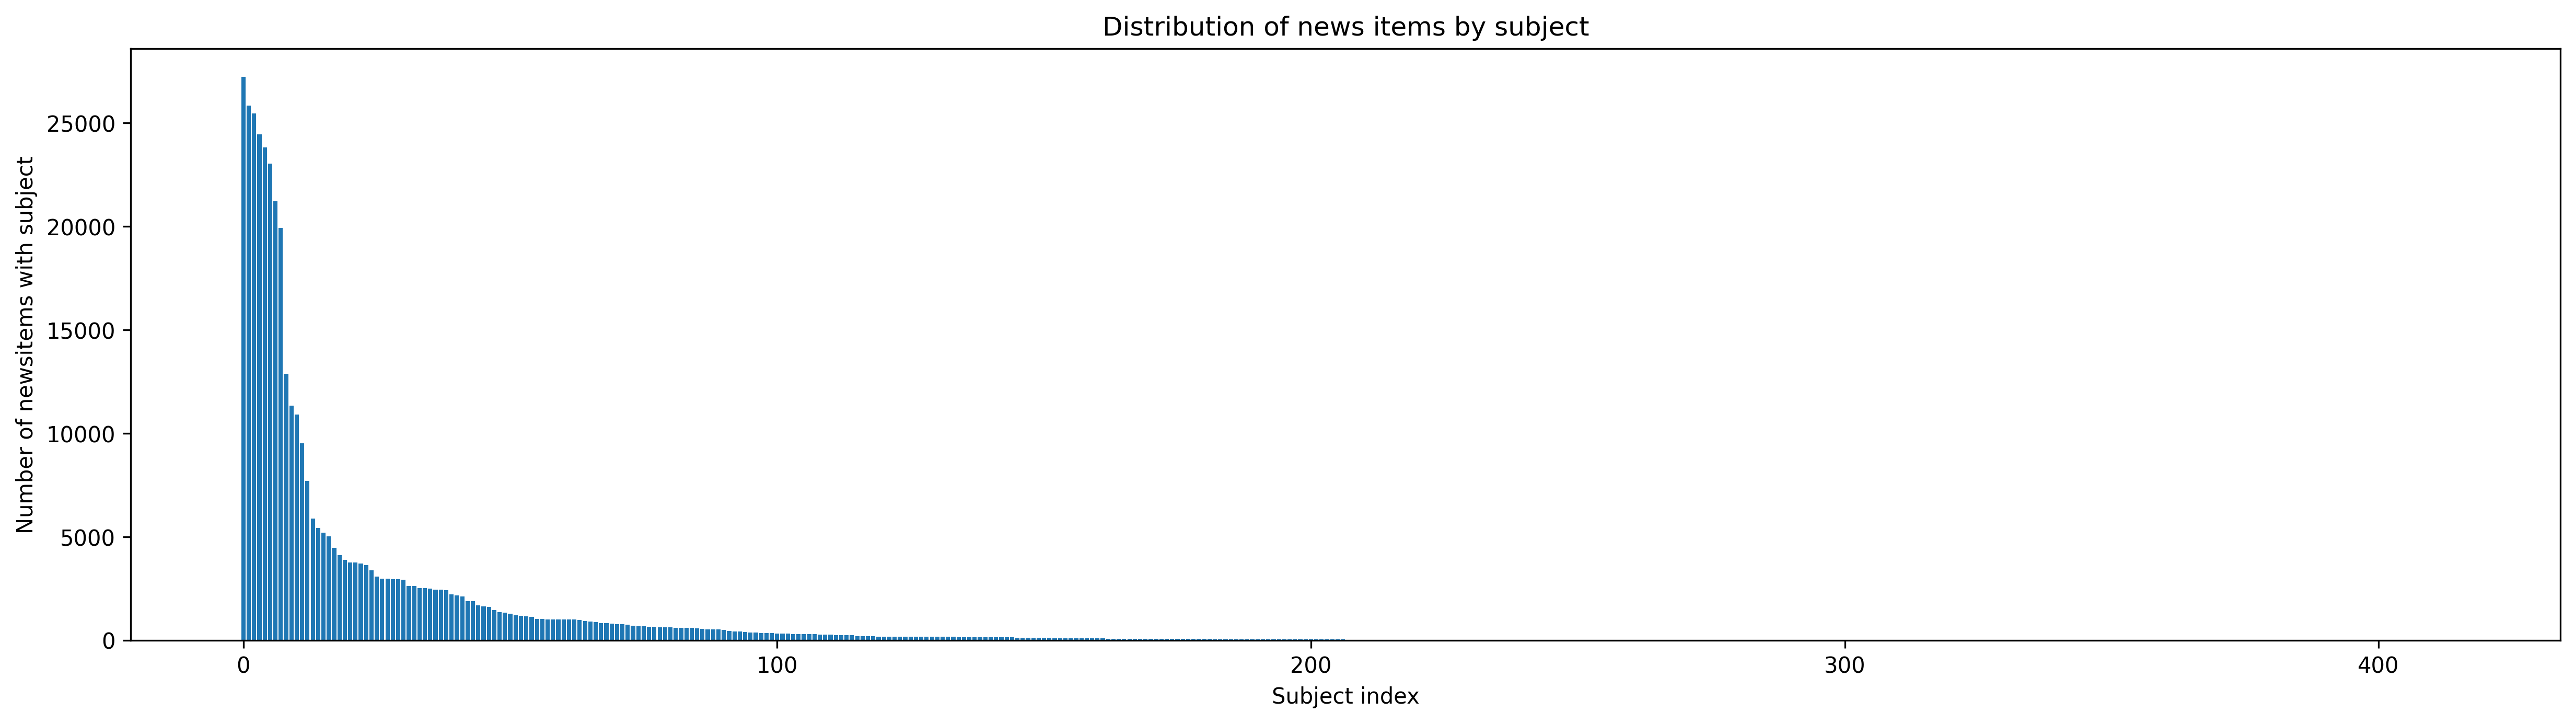
\includegraphics[scale=0.35]{distribution_news_item_subject}}
      \caption{\textit{Distribution of news items by subject}}
    \end{figure}

    \begin{figure}
      \centerline{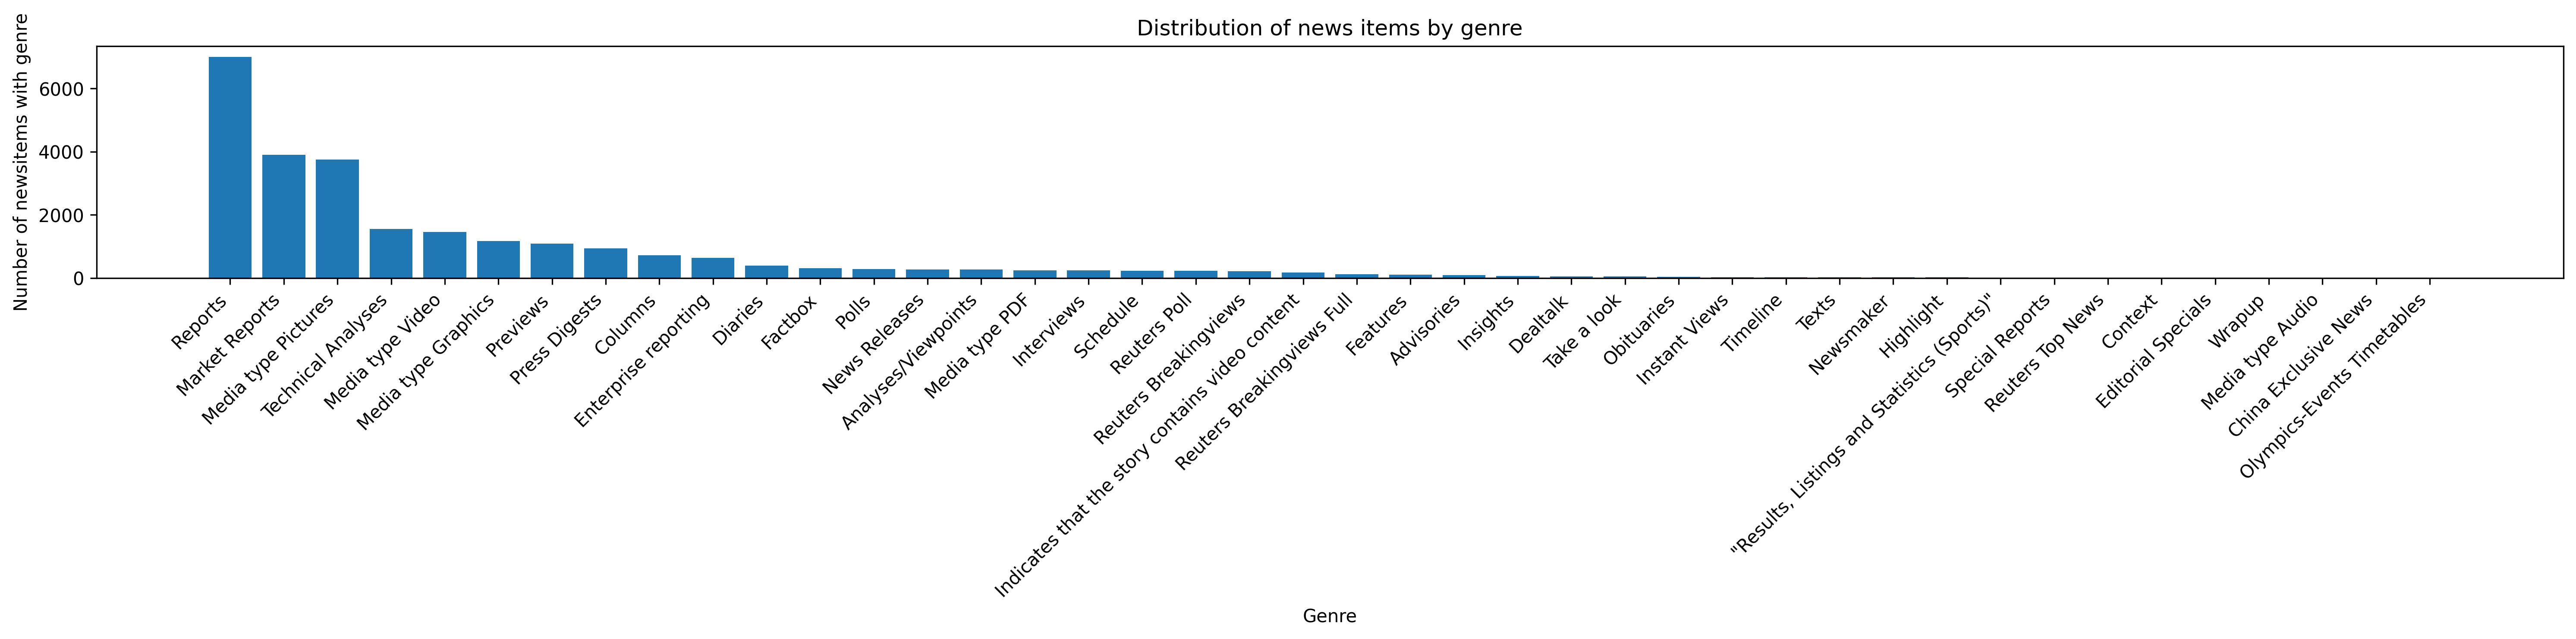
\includegraphics[scale=0.3]{distribution_news_item_genre}}
      \caption{\textit{Distribution of news items by genre}}
    \end{figure}

    }
  \end{itemize}
  (see\hyperref[sec:AppendixB]{``Appendix B"})
  
  \subsubsection{Data challenges}
  Cleaning this dataset presented a few unique challenges, which will be considered in the NLP section below.
  \begin{itemize}
    \item{This corpus included some XML documents with unique encoding issues between UTF-8 encoding and plain text. For example, some of the XML documents\footnote{tag:reuters.com,2019:newsml\_CqtHM2P1a} included Tweets with emojis. A future effort could handle such emojis more gracefully. Furthermore, some apostrophes were transformed \footnote{For example, headline ``BREAKINGVIEWS-Carmakers,\"A\^o antitrust probe is more smoke than fire" (tag:reuters.com,2019:newsml\_L2N25X0YW).}
    }
    \item{Some documents include table-formatted text, with many spaces meant to be rendered in a monospace format. In this case, a simple logic to consider a single space as a word boundary is not correct.\footnote{For example, item tag:reuters.com,2019:newsml\_L3N2602HC:991614233 should not be considered to have 76,783 words. It has 294,233 spaces when counting all whitespace, but this is a table-formatted item, not a long piece of text.}}
    \item{Some documents are incredibly long direct quotations transcribed from an event. These should be handled differently than other news reports.\footnote{For example, item tag:reuters.com,2019:newsml\_CqtYP8GSa:1548902168.XML is a full transcript of a committee hearing on US-China relations.}}
  \end{itemize}

  \subsubsection{Graph database ingestion (\lstinline{csvs_to_neo4j.cypher})}
  Finally, the CSVs were combined and ingested into Neo4g as a graph database. Cypher queries were run to ingest the primary metadata from each cleaned XML news item into Neo4j as a property graph with initial relationships (see\hyperref[sec:AppendixC]{``Appendix C"}). After running these Cypher queries, a prototype knowledge graph is available for meaningful queries and initial information retrieval (see\hyperref[sec:DataSetEvaluation]{``Data Set Evaluation"} below). This step uses Neo4j, Cypher, and APOC to load the cleaned CSV, create Neo4j nodes for each NewsItem, Subject, and Genre, add properties to the nodes, and create \lstinline{-[:HAS_GENRE]->} and \lstinline{-[:HAS_SUBJECT]->} relationships.



\subsection{Data Set Evaluation}
\label{sec:DataSetEvaluation}

With the data sourcing, cleaning, and graph database ingestion complete, we can evaluate the raw data and begin to see the practical value of a knowledge graph in terms of information retrieval.

At a basic level, the overall shape of the data and graph become clear. As shown in \textit{Table 2} and \textit{Table 3}, nearly 60,000 nodes are now available in the Neo4j graph database. Furthermore, there is interesting variance in the number of relationships per node, while keeping the properties per node constant across all NewsItems, Genres, and Subjects.


\begin{table}
  \begin{tabular}{ |p{3cm}||p{2cm}|p{7cm}|  }
  \hline
  \multicolumn{3}{|c|}{Neo4j Knowledge Graph Nodes: high-level view of graph DB schema} \\
  \hline
  Node (Label)& Count &Properties\\
  \hline
  NewsItem&59,542&guid, filename, headline, slugline, datetime, genres, bodyLengthWords, subjects, description, bodyLengthChars, bodyLengthCharsNonWhitespace\\
  \hline
  Subject&414&category, subject, wikidataURL, wikipediaURL\\
  \hline
  Genre&42&genre\\
  \hline
  \end{tabular}
  \caption{\textit{Initial Knowledge Graph overview}}
\end{table}

\begin{table}
  \begin{lstlisting}
  MATCH (n)
  WITH labels(n) as labels, size(keys(n)) as props, size((n)--()) as degree
  RETURN
  DISTINCT labels,
  count(*) AS NumNodes,
  avg(props) AS AvgNumPropPerNode,
  min(props) AS MinNumPropPerNode,
  max(props) AS MaxNumPropPerNode,
  avg(degree) AS AvgNumRelationships,
  min(degree) AS MinNumRelationships,
  max(degree) AS MaxNumRelationships
  \end{lstlisting}

  \begin{tabular}{ |p{2cm}|p{1cm}|p{1.5cm}|p{1.5cm}|p{1.5cm}|p{1.5cm}|p{1.5cm}|p{1.5cm}| }
  \hline
  labels&Num-Nodes&AvgNum-PropPer-Node&MinNum-PropPer-Node&MaxNum-PropPer-Node&AvgNum-Relation-ships&MinNum-Relation-ships&MaxNum-Relation-ships\\
  \hline
  [``NewsItem"]&59542&11&11&11&7.55&0&94\\
  \hline
  [``Genre"]&42&1&1&1&618.31&1&7250\\
  \hline
  [``Subject"]&415&5&5&5&1021.13&0&27250\\
  \hline
  \end{tabular}

  \caption{\textit{Cypher query\protect \footnotemark to inventory initial nodes and relationships in the knowledge graph}}
\end{table}

\footnotetext{\url{https://neo4j.com/developer/kb/how-do-i-produce-an-inventory-of-statistics-on-nodes-relationships-properties/}}


More significantly, at this point the knowledge graph's practical value begins to become evident, as some human-interpretable queries are now possible, which were not originally possible with the raw data. Whereas the unstructured collection of semi-structured XML documents could not be queried, now we can present meaningful queries over the dataset, including the following\footnote{some of these are available in \lstinline{query_ky.cypher}...potentially to include in Appendix}:

\begin{itemize}
  \item{Finding all news items that have two specific subjects or all items that have more than a certain number of genre or subject relationships (see \textit{Figure 3}).}
  \item{Finding the shortest news items and longest news items by length in characters (see \textit{Figure 4}).}
  \item{Finding the subjects and genres assigned to the most items (see \textit{Figure 5}). Note that these figures confirm what was already discovered in the distribution findings of \textit{Figure 1} and \textit{Figure 2}.}
  \item{Finding the shortest path between two items, perhaps to quickly see what some news stories have in common (see \textit{Figure 6}).}
\end{itemize}


\begin{figure}
  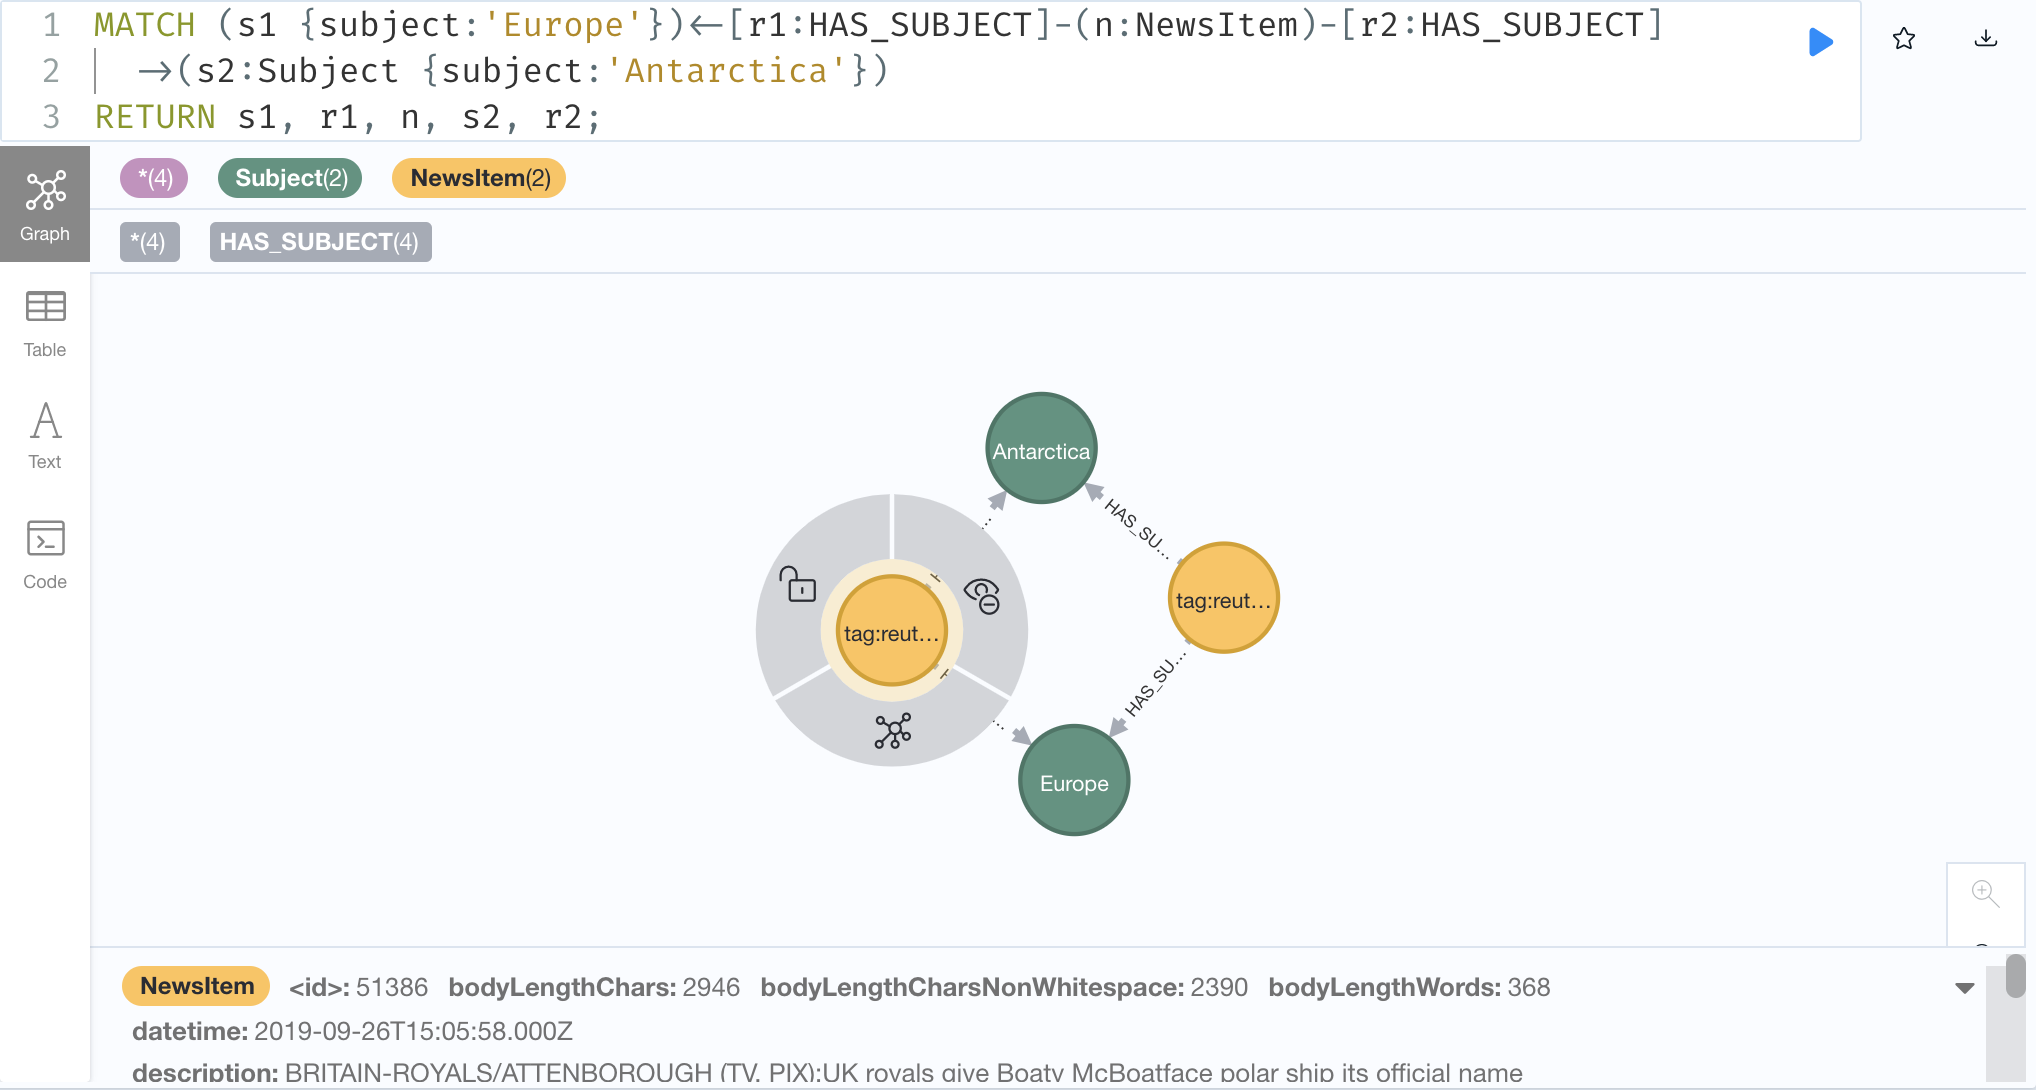
\includegraphics[scale=0.2]{00-news-items-antarctica-europe}
  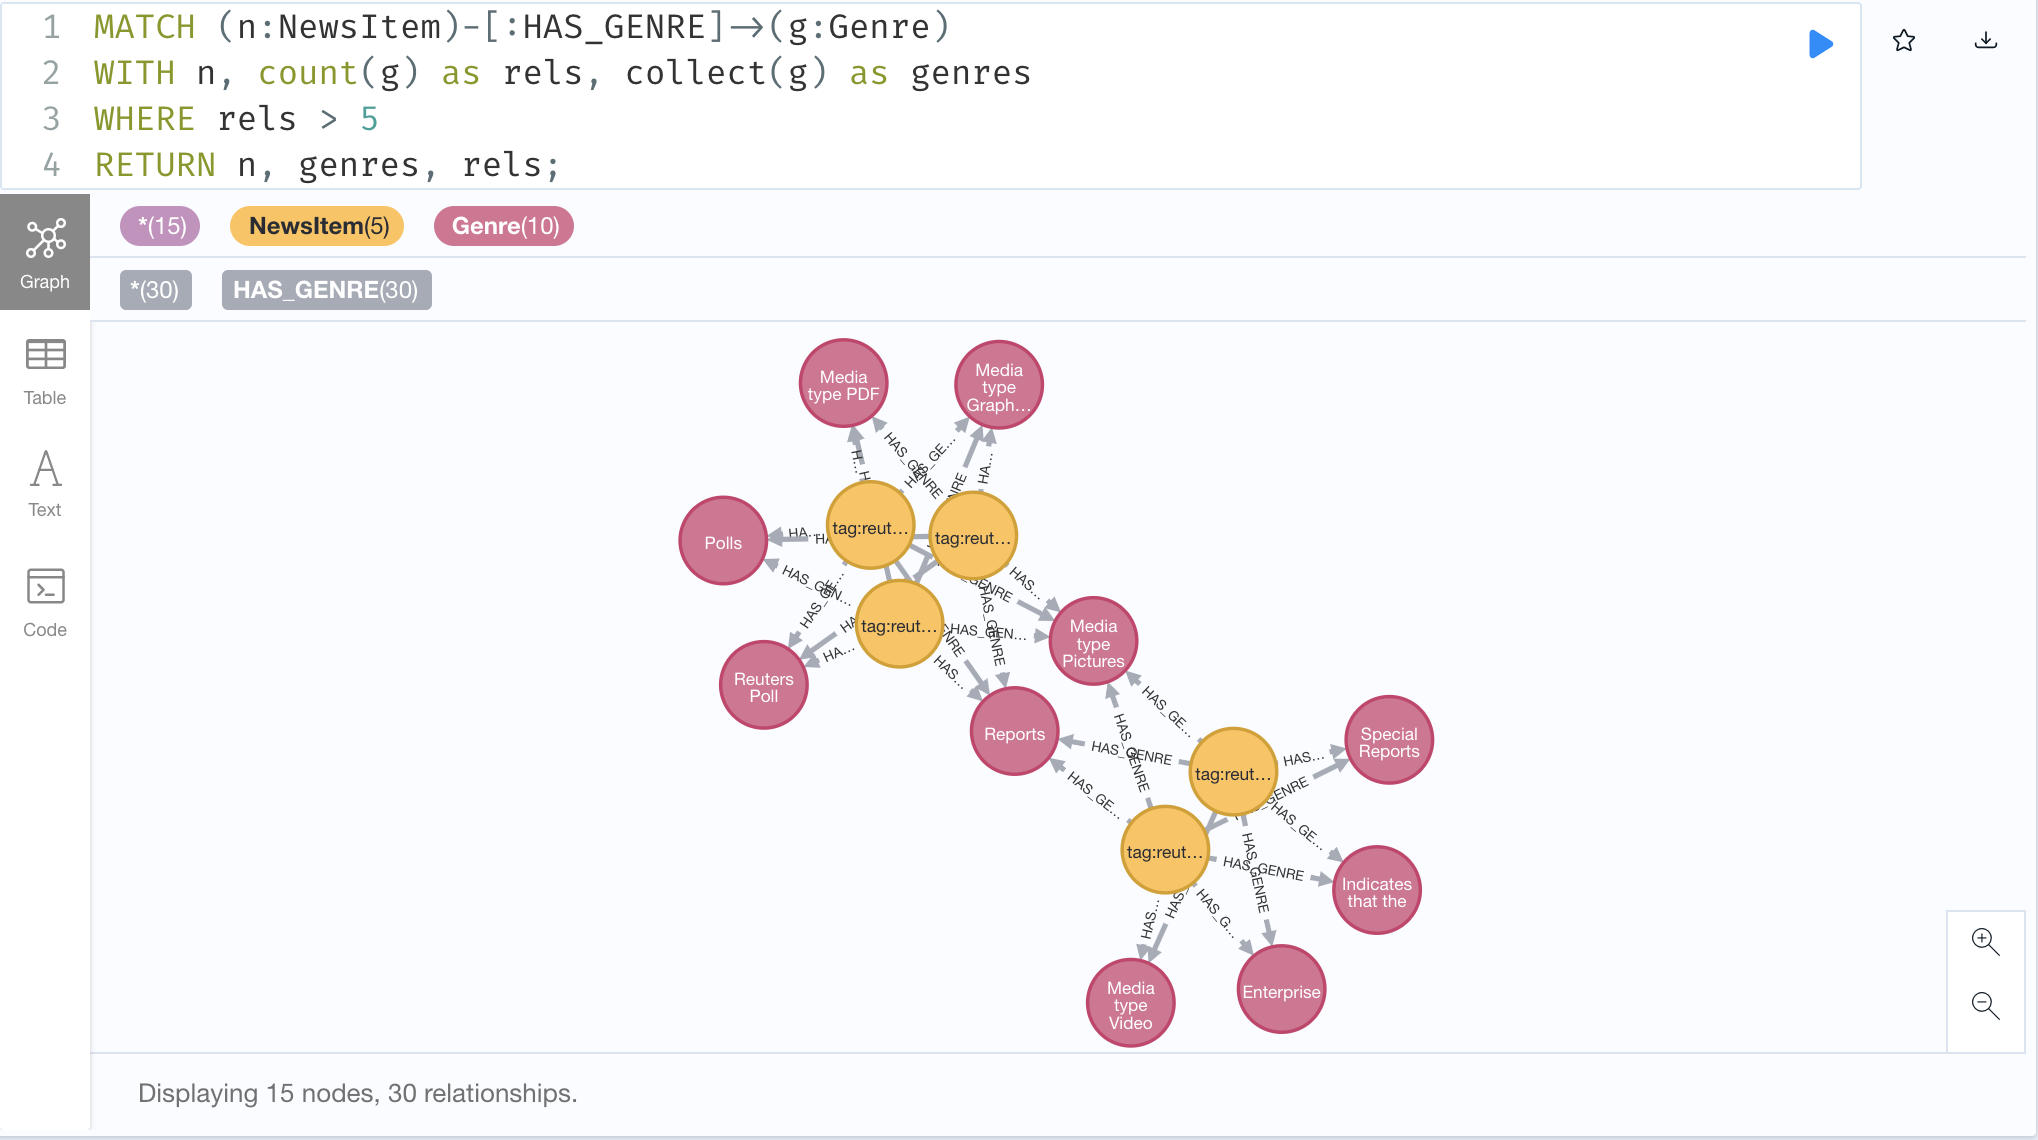
\includegraphics[scale=0.2]{00-news-items-more-than-five-genres}
  \caption{\textit{Knowledge graph Cypher queries: subject and genre relationships)}}
\end{figure}

\begin{figure}
  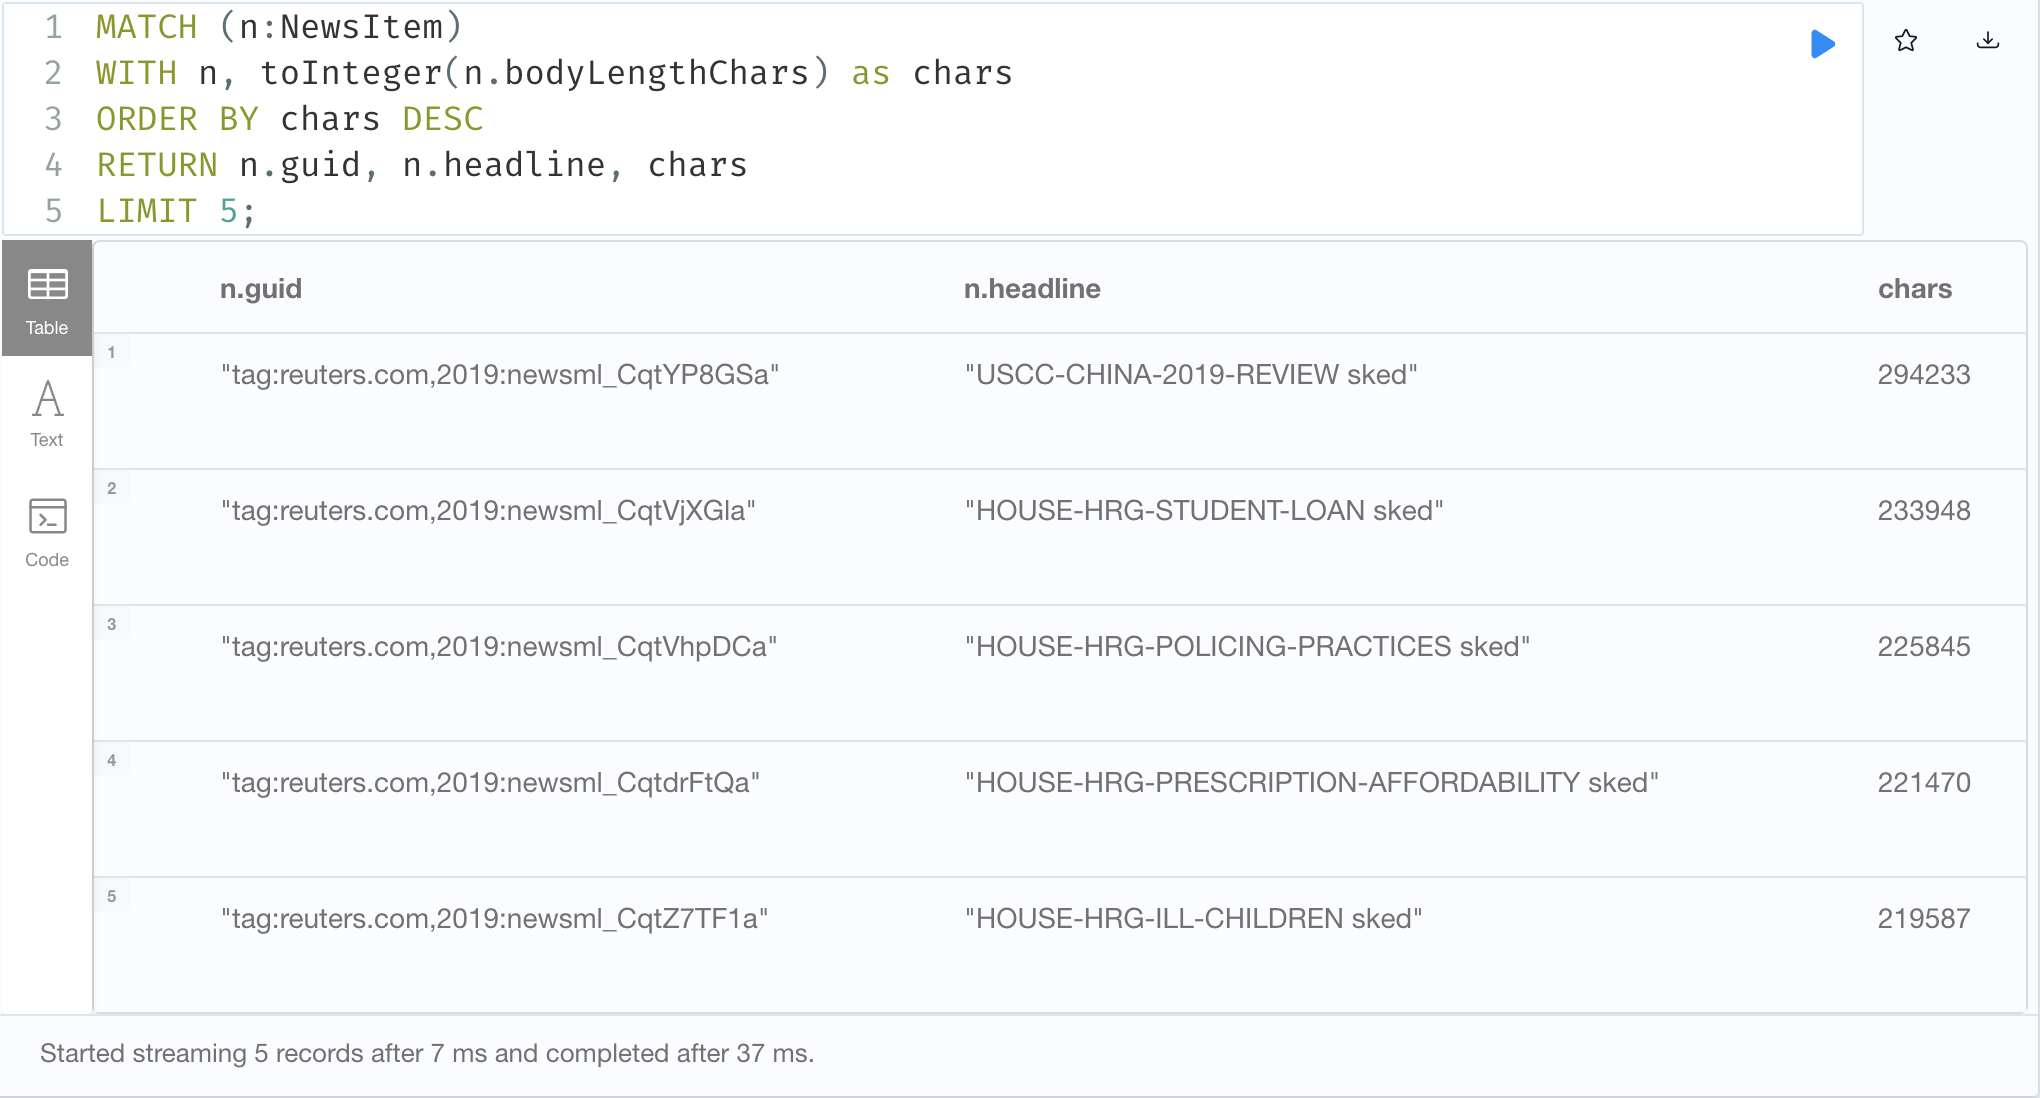
\includegraphics[scale=0.2]{01-longest-items}
  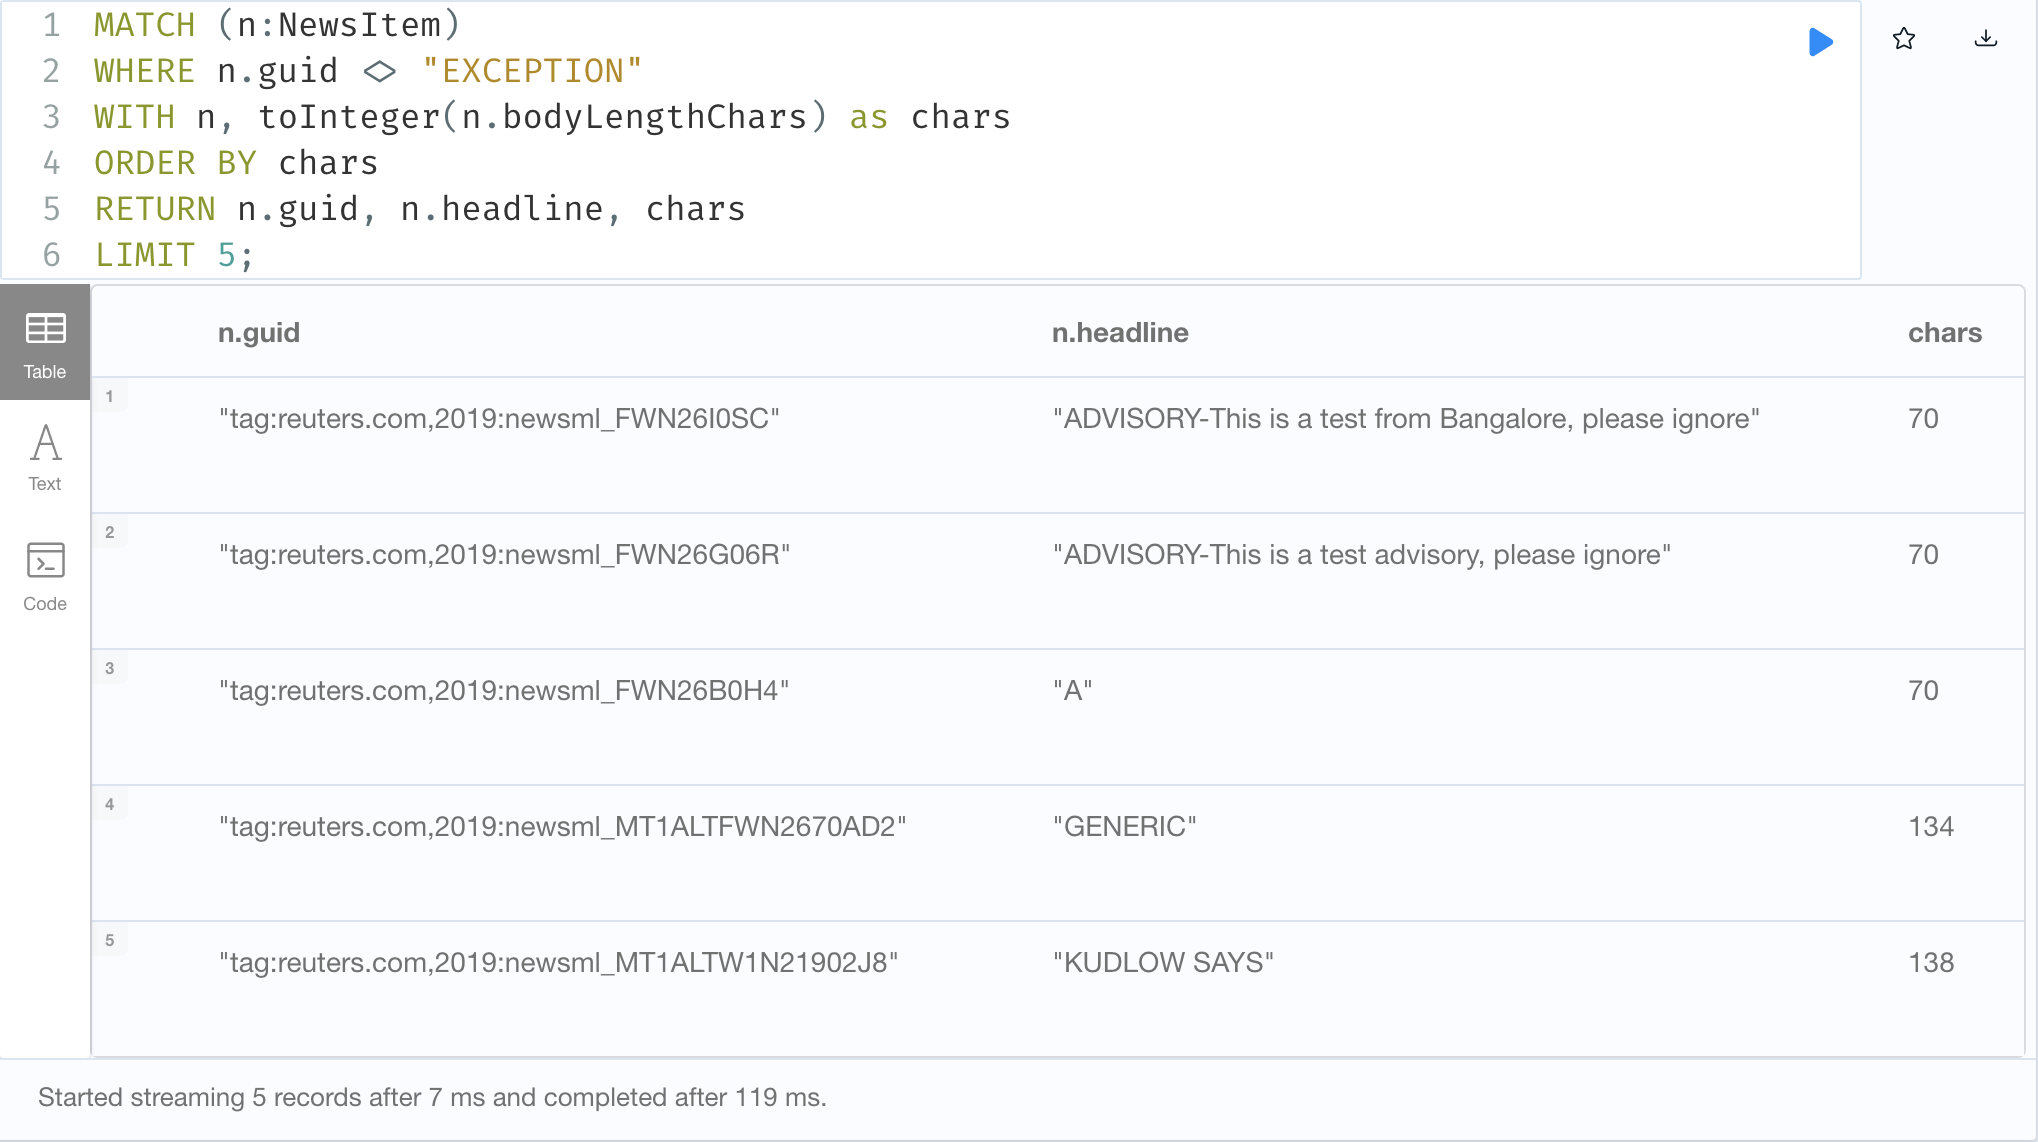
\includegraphics[scale=0.2]{01-shortest-items}
  \caption{\textit{Knowledge graph Cypher queries: shortest and longest news text}}
\end{figure}

\begin{figure}
  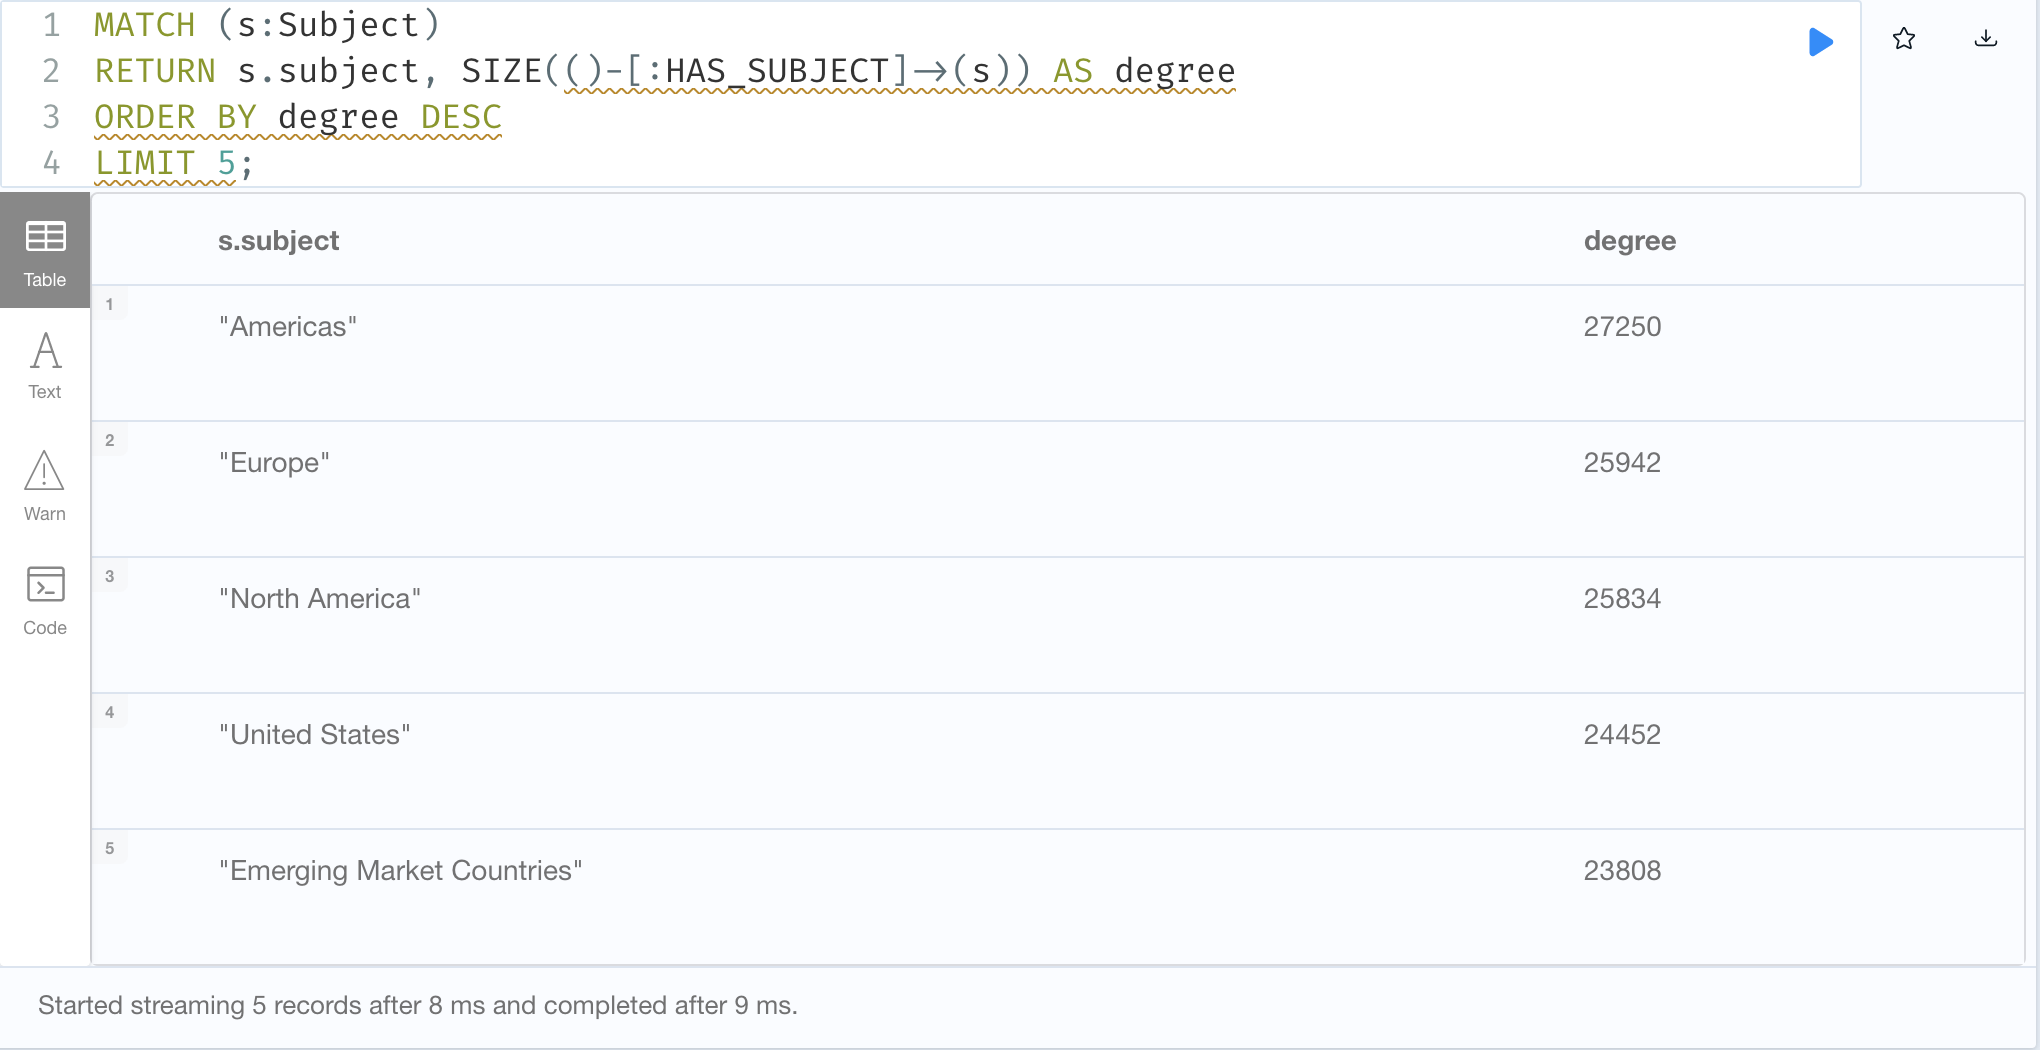
\includegraphics[scale=0.2]{02-subjects-with-most-items}
  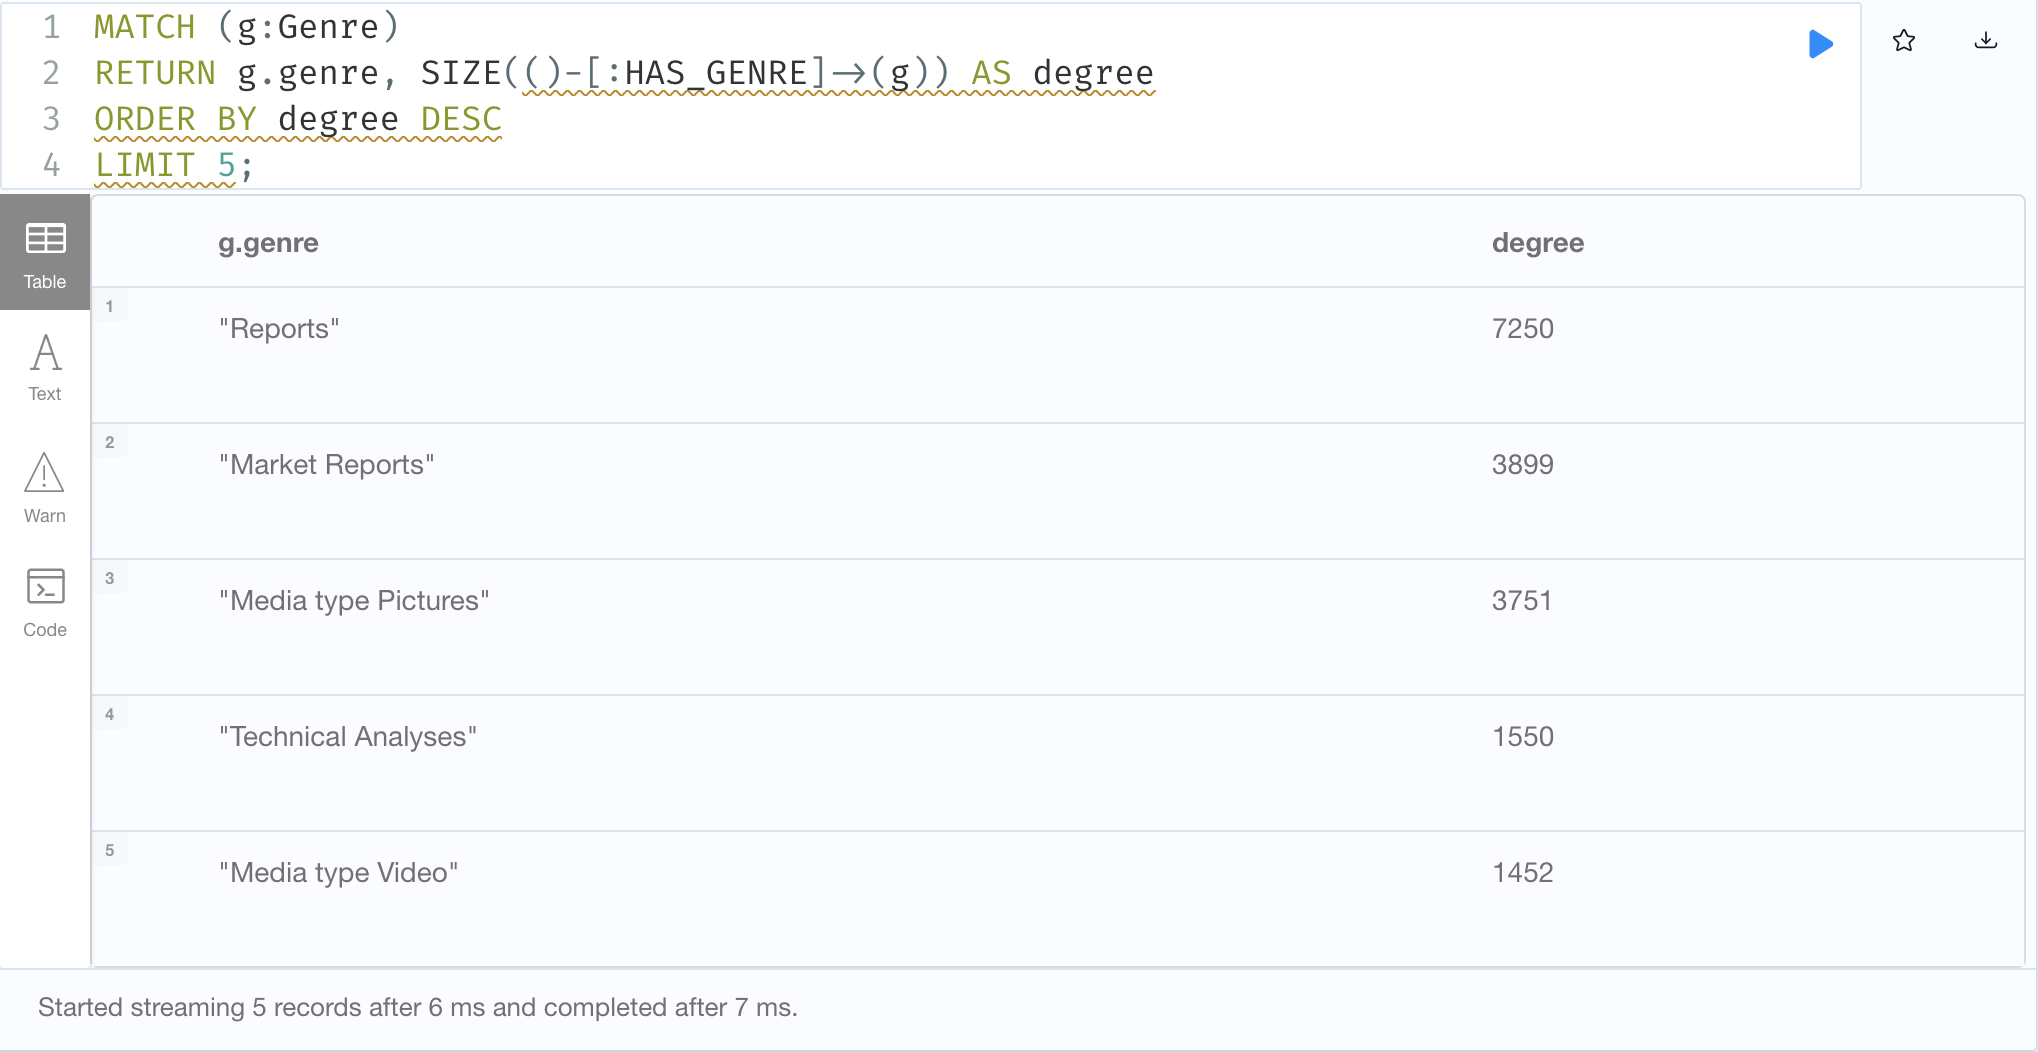
\includegraphics[scale=0.2]{02-genres-with-most-items}
  \caption{\textit{Knowledge graph Cypher queries: subjects and genres with most items}}
\end{figure}

\begin{figure}
  \centerline{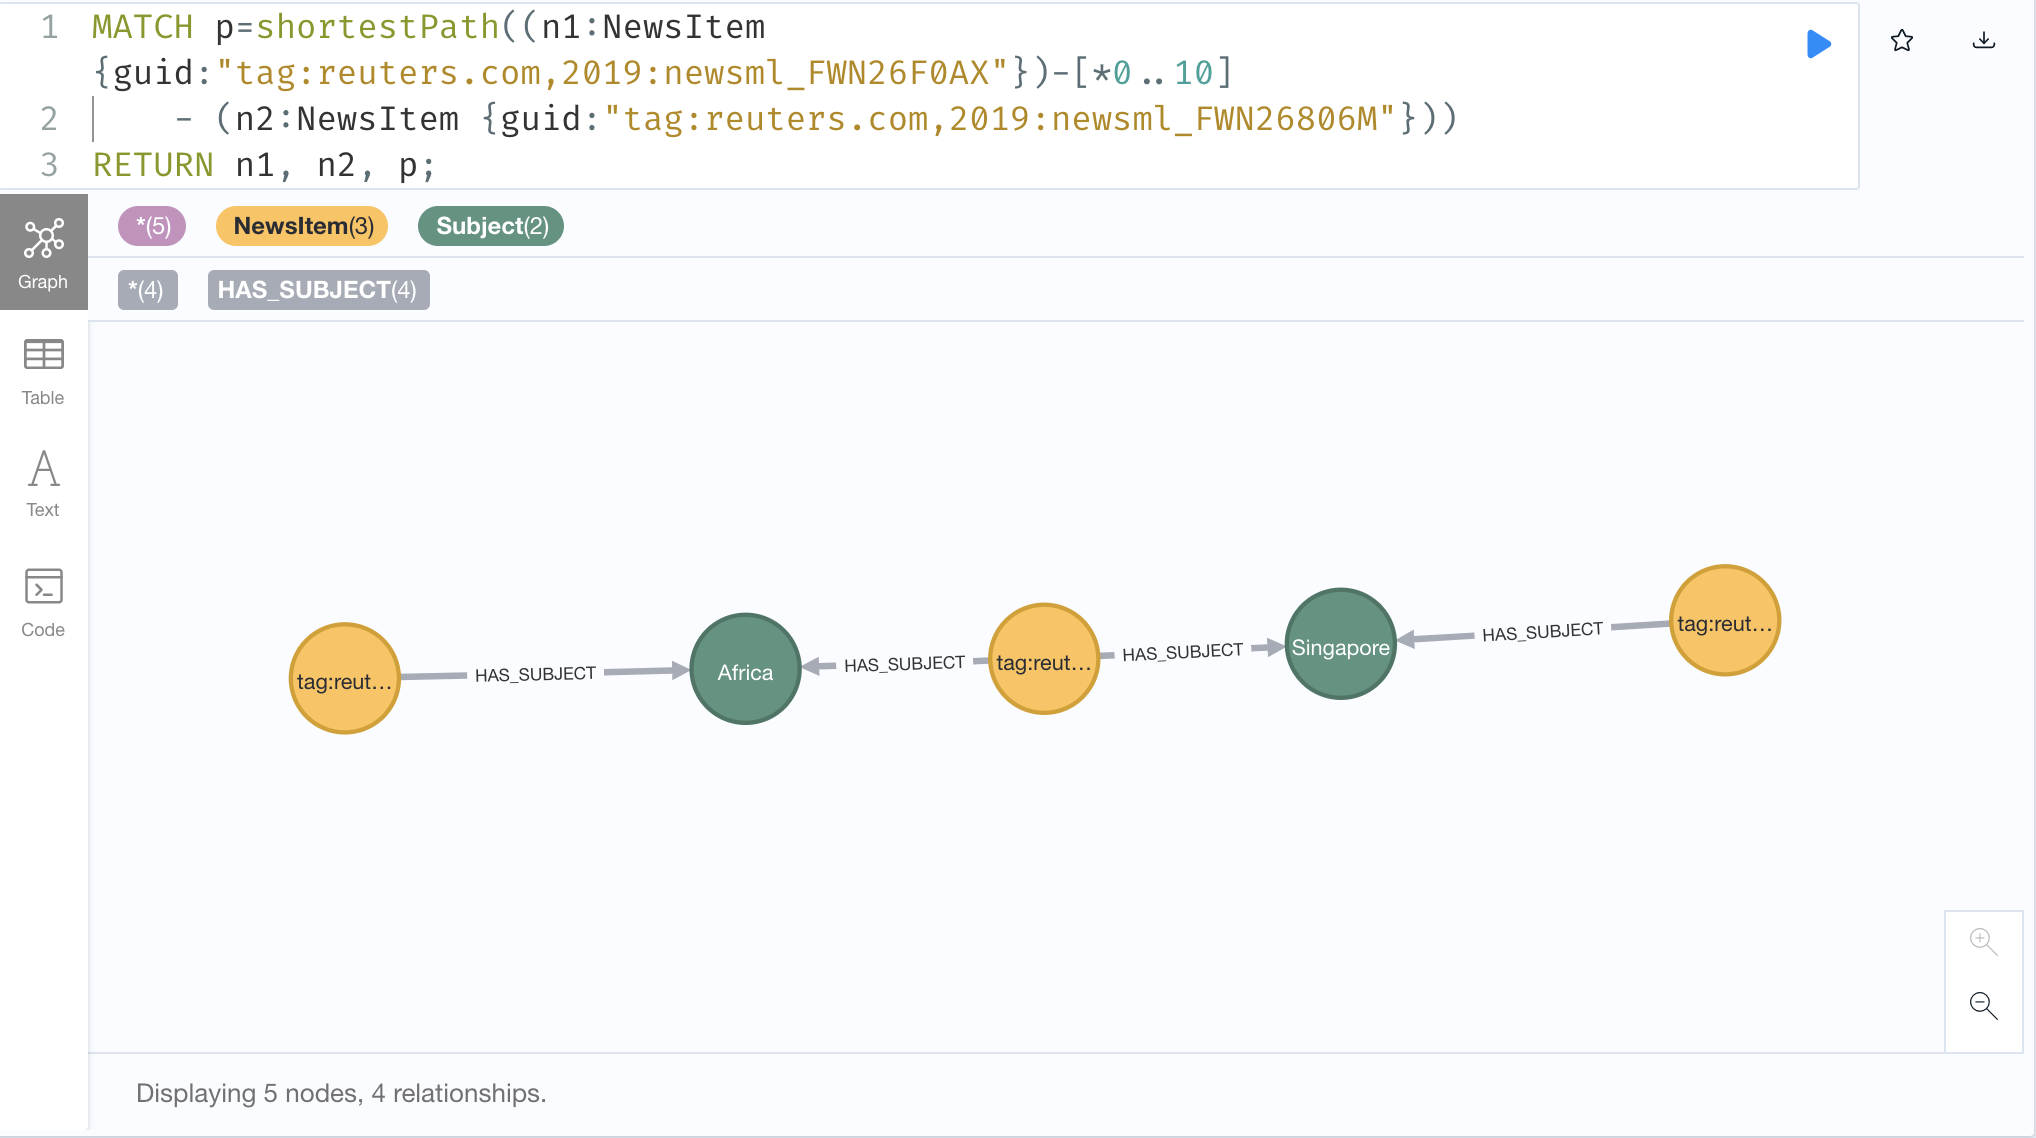
\includegraphics[scale=0.2]{03-shortest-path}}
  \caption{\textit{Knowledge graph Cypher queries: shortest path}}
\end{figure}


\section{Knowledge Graph Design and Enhancement}

Building on the domain-sepcific knowledge graph of news items from the previous sections, the analysis now focuses on enhancements to the knowledge graph. This includes (1) semantic enhancements using ontologies and linked data; (2) NLP enhancements to extract entities and other meaning from the English language text; and (3) network analysies around centrality, clustering, and betweenness. It draws guidance and technical examples from Neo4j's developer guides\footnote{\url{https://neo4j.com/developer/}}, including the Neo4j knowledge graph tutorial\cite{neo4j-kg-tutorial}.

\subsection{Semantic Enhancements}

Neo4j has a useful plugin called neosemantics (n10s), which "enables the use of RDF and its associated vocabularies like (OWL,RDFS,SKOS and others) in Neo4j" \footnote{https://neo4j.com/labs/neosemantics/}. This makes n10s a suitable technology for semantic enhancements of the news knowledge graph.

For this knowledge graph, Wikidata\footnote{https://www.wikidata.org/} was chosen as the knowledge base to link with the published news documents. After reflecting on the content of the Reuters news items, it became clear that a few resource types are commonly present in news items:
\begin{itemize}
  \item{Geography (countries, cities)}
  \item{People (politicians, athletes)}
  \item{Organisations (political parties, companies)}
\end{itemize}

SPARQL queries can find the Wikidata category for each of these and recursively identify the subcategories. By importing these categories and subcategories in an RDF subject-predicate-object format with n10s, the Neo4j knowledge graph can represent the relationships between parent/child categories and instances of specific categories.

For example:
\begin{lstlisting}
  WITH "https://query.wikidata.org/sparql?query=..." AS uri
  CALL n10s.rdf.import.fetch(uri, 'Turtle' , { headerParams: { Accept: "application/x-turtle" } })
  YIELD terminationStatus, triplesLoaded, triplesParsed, namespaces, callParams
  RETURN terminationStatus, triplesLoaded, triplesParsed, namespaces, callParams;

  MATCH path = (c:Category {name: "republic"})<-[:SUB_CAT_OF*]-(child)
  RETURN path
  LIMIT 25;
\end{lstlisting}

\begin{figure}
  \centerline{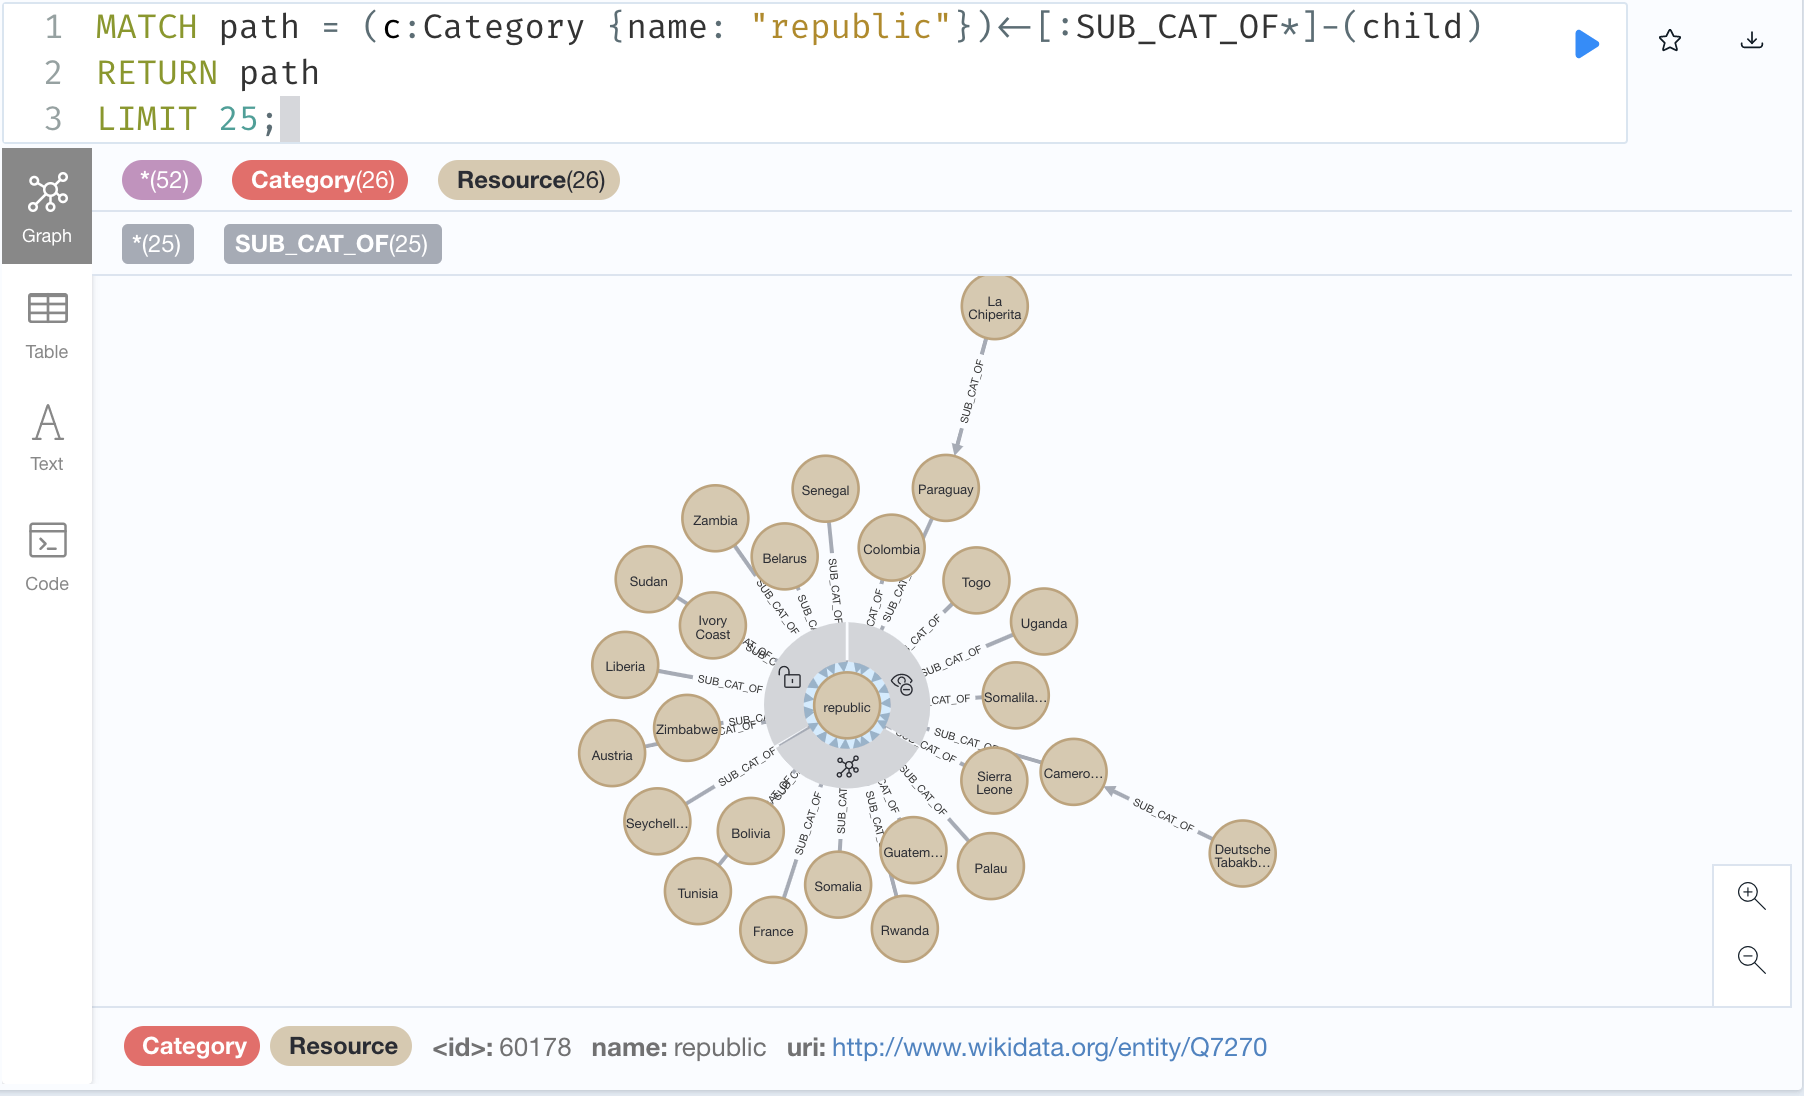
\includegraphics[scale=0.5]{category-republic.png}}
  \caption{\textit{Countries which are instances of republic}}
\end{figure}

This provides a foundation of knowledge via Wikidata's ontology, which can now be connected to facts from the news items via natural language processing (NLP) and entity extraction.

\subsection{Natural Language Processing}

The APOC plugin enables Neo4j Cypher queries to use the Google Cloud Platform's entity extraction procedures\footnote{\url{https://neo4j.com/labs/apoc/4.1/nlp/gcp}}.

By running entity extraction over each news item's text body, which takes approximately 10 hours for all 59,542 items, we can now see entities for a given news item. For example, a news item about the Gap clothing company may have entities United States, Gap, and Sephora (see "Figure 12").

\begin{figure}
  \centerline{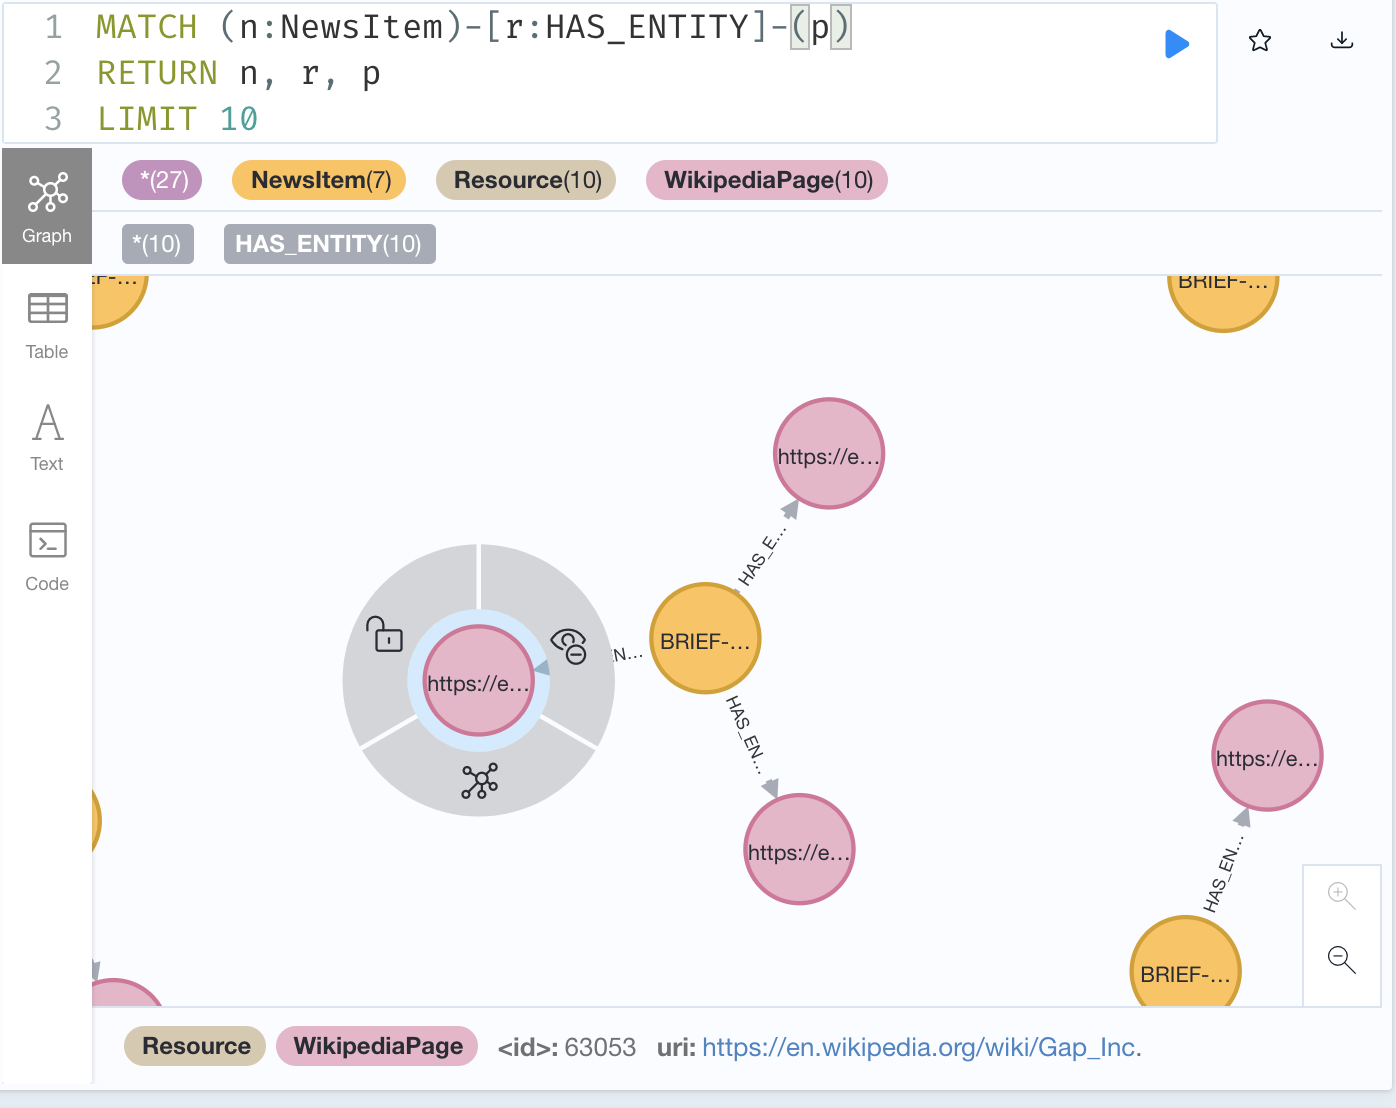
\includegraphics[scale=0.5]{has-entity.png}}
  \caption{\textit{\lstinline{(n:NewsItem)-[:HAS_ENTITY]->(p:WikipediaPage)}}}
\end{figure}

\subsection{Models, networks, etc.???}

Clustering, betweenness

\section{[WIP] Evaluation}

(Note to self: see evaluation.md)

% \subsection{Interpretability}
% \subsection{Others...confusion matrix, predictions, clustering, betweenness, etc.}

\section{[WIP] Conclusions}
\subsection{Future Work}
\subsection{Conclusion}


\newpage

\section{Appendix}
\subsection{Appendix XML...}
\label{sec:AppendixXML}
Sample XML document from Reuters corpus on AWS S3, specifically file \lstinline{tag/reuters.com,2019/newsml_L2N25V1DP/702697965}:
\\


\begin{lstlisting}[basicstyle=\tiny]
<?xml version="1.0" encoding="UTF-8"?>
<!-- 
SUMMARY: 
- Structure: NML2 SNI Text 
- Based On: NML2 v2.10

AUTHOR: thomsonreuters.com
-->
<!-- ========================================================= -->
<newsMessage xmlns="http://iptc.org/std/nar/2006-10-01/" xmlns:rtr="http://www.reuters.com/ns/2003/08/content" xmlns:x="http://www.w3.org/1999/xhtml" xmlns:xsi="http://www.w3.org/2001/XMLSchema-instance">
  <header>
    <sent>2019-09-04T20:08:51.000Z</sent>
    <sender>reuters.com</sender>
    <transmitId>tag:reuters.com,2019:newsml_L2N25V1DP:702697965</transmitId>
    <priority>3</priority>
  </header>
  <itemSet>
    <newsItem conformance="power" guid="tag:reuters.com,2019:newsml_L2N25V1DP" standard="NewsML-G2" standardversion="2.10" version="702697965" xml:lang="en">
      <catalogRef href="http://www.iptc.org/std/catalog/catalog.IPTC-G2-Standards_3.xml"/>
      <rightsInfo>
        <copyrightHolder literal="Thomson Reuters"/>
        <copyrightNotice xml:lang="en">(c) Copyright Thomson Reuters 2019. Click For Restrictions - https://agency.reuters.com/en/copyright.html</copyrightNotice>
      </rightsInfo>
      <itemMeta>
        <itemClass qcode="icls:text" rtr:msgType="S"/>
        <provider literal="reuters.com"/>
        <versionCreated>2019-09-04T20:08:51.000Z</versionCreated>
        <firstCreated>2019-09-04T20:08:51.000Z</firstCreated>
        <pubStatus qcode="stat:usable"/>
        <role qcode="itemRole:N"/>
        <fileName>2019-09-04T200851Z_702697965_L2N25V1DP_RTRMADT_0_EXXON-MOBIL-CHEVRON-BREAKINGVIEWS.XML</fileName>
        <generator versioninfo="1.0.0.21">LYNX:addT:001</generator>
        <profile versioninfo="00.00.01">SNI-Text</profile>
        <service qcode="svc:RTR_TNS"/>
        <instanceOf qcode="NI:CURRIE/"/>
        <signal qcode="edStat:N"/>
        <rtr:versionedId guid="tag:reuters.com,2019:newsml_L2N25V1DP:702697965"/>
      </itemMeta>
      <contentMeta>
        <urgency>3</urgency>
        <infoSource literal="Reuters" qcode="NS:RTRS" role="cRole:origProv"/>
        <creator literal="Reuters"/>
        <altId rtr:isOriginal="1" type="idType:EAID">23b9e59f-48cf-e911-718c-215056936dab</altId>
        <language tag="en"/>
        <subject qcode="N2:US" type="cptType:5">
          <name>United States</name>
          <facet qcode="geoProp:5"/>
        </subject>
        <subject qcode="N2:NAMER" type="cptType:5">
          <name>North America</name>
          <facet qcode="geoProp:3"/>
        </subject>
        <genre qcode="N2:BRV">
          <name>Reuters Breakingviews</name>
        </genre>
        <slugline separator="-">EXXON MOBIL-CHEVRON/BREAKINGVIEWS</slugline>
        <headline>BREAKINGVIEWS-Exxon CEO risks fueling unholy investor alliance</headline>
        <creditline>Reuters</creditline>
        <description role="descRole:caption">EXXON MOBIL-CHEVRON/BREAKINGVIEWS:BREAKINGVIEWS-Exxon CEO risks fueling unholy investor alliance</description>
        <by>By Antony Currie</by>
      </contentMeta>
      <assert qcode="R:XOM.N">
        <name>Exxon Mobil Corp</name>
        <sameAs qcode="NDAID:36999"/>
        <organisationDetails>
          <rtr:companydata exchange="NYS" exchangecv="MDNA" name="Exxon Mobil Corp" ric="XOM.N" tickersymbol="XOM"/>
        </organisationDetails>
      </assert>
      <contentSet>
        <inlineXML contenttype="application/xhtml+html" wordcount="209">
          <html xmlns="http://www.w3.org/1999/xhtml">
            <head>
              <title/>
            </head>
            <body>
              <p>(The author is a Reuters Breakingviews columnist.  The opinions
expressed are his own.)</p>
              <p>By Antony Currie</p>
              <p>NEW YORK, Sept 4 (Reuters Breakingviews) - Darren Woods
reckons human progress and the unreliability of alternative
energy sources justifies investing more in emissions-laden
fossil fuels. But his argument ignores the $293 bln driller's
poor returns. That may give financial investors common cause
with climate activists...</p>
            </body>
          </html>
        </inlineXML>
      </contentSet>
    </newsItem>
  </itemSet>
</newsMessage>
\end{lstlisting}
\newpage

\subsection{Appendix A. \textit{\lstinline{item_xml_docs_to_csv.py}} to transform XML docs to CSV}
\label{sec:AppendixA}
Save the following code as \textit{\lstinline{item_xml_docs_to_csv.py}} and run using command line arguments below with a directory of XML / NewsMLG2 documents.
\\

\begin{lstlisting}[language=Python, basicstyle=\tiny]
import csv
import os
import re
import sys
import xml.etree.ElementTree as ET


NSMAP = {'iptc': 'http://iptc.org/std/nar/2006-10-01/',
         'xhtml': 'http://www.w3.org/1999/xhtml'}
CSV_ROW_LIMIT = 10000
VERBOSE = False

# workaround solution for encoded emojis in tweets
% INVALID_CHAR_REGEX = '&#\d\d\d\d\d;'

def save_to_csv(news_items, filename):
  fields = ['filename',
            'datetime',
            'guid',
            'slugline',
            'headline',
            'description',
            'genres',
            'subjects',
            'bodyLengthChars',
            'bodyLengthCharsNonWhitespace',
            'bodyLengthWords',
            # 'body'
            ]

  with open(filename, 'w') as csvfile:
    writer = csv.DictWriter(csvfile, fieldnames=fields)
    writer.writeheader()
    writer.writerows(news_items)

def make_news_item_dict(filename, body='', datetime='EXCEPTION', description='EXCEPTION',
                        genres='EXCEPTION', guid='EXCEPTION', headline='EXCEPTION',
                        slugline='EXCEPTION', subjects='EXCEPTION'):
  """
  Return dictionary of news_item. For empty case (in exceptions), default arguments
  will be 'EXCEPTION' and 0 length for bodyLengthChards and bodyLengthWords.
  """
  return {#'body': body,
          'datetime': datetime,
          'description': description,
          'filename': filename,
          'genres': genres,
          'guid': guid,
          'headline': headline,
          'slugline': slugline,
          'subjects': subjects,
          'bodyLengthChars': len(body),
          'bodyLengthCharsNonWhitespace': len(body.replace(' ', '')),
          'bodyLengthWords': len(re.split('\s+', body))} # split on \s+ for one *or more* spaces

def parse_xml(path, filename):
  file = path + '/' + filename
  try:
    root = ET.parse(file).getroot()
  except Exception as e:
    raise(e)
    with open(file, 'r') as file:
      data = file.read()
      data = re.sub(INVALID_CHAR_REGEX, '', data)
      root = ET.fromstring(data)

  guid = root.find('./iptc:itemSet/iptc:newsItem', namespaces=NSMAP).get('guid')

  subject_nodes = root.findall('./iptc:itemSet/iptc:newsItem/iptc:contentMeta/iptc:subject/iptc:name',\
                               namespaces=NSMAP)
  subjects = set()
  if len(subject_nodes) == 0:
    subjects = None
  else:
    for s in subject_nodes:
      subjects.add(s.text)

  genre_nodes = root.findall('./iptc:itemSet/iptc:newsItem/iptc:contentMeta/iptc:genre/iptc:name',\
                             namespaces=NSMAP)
  if len(genre_nodes) == 0:
    genres = None
  else:
    genres = set()
    for g in genre_nodes:
      genres.add(g.text)

  datetime = root.find('./iptc:itemSet/iptc:newsItem/iptc:itemMeta/iptc:firstCreated', namespaces=NSMAP).text
  slugline = root.find('./iptc:itemSet/iptc:newsItem/iptc:contentMeta/iptc:slugline',\
                       namespaces=NSMAP).text
  headline = root.find('./iptc:itemSet/iptc:newsItem/iptc:contentMeta/iptc:headline',\
                       namespaces=NSMAP).text
  description = root.find('./iptc:itemSet/iptc:newsItem/iptc:contentMeta/iptc:description',\
                          namespaces=NSMAP).text
  body = root.find('./iptc:itemSet/iptc:newsItem/iptc:contentSet/iptc:inlineXML/xhtml:html/xhtml:body',\
                   namespaces=NSMAP)#.text
  body = str(ET.tostring(body))

  return make_news_item_dict(filename, body, datetime, description, genres, guid,\
                             headline, slugline, subjects)

def parse_xml_and_write_csv(path, files, output_filename):
  counter = 0
  news_items = []
  n_files = len(files)
  check_length = n_files // 10 + 1
  for i, filename in enumerate(files):
    if VERBOSE:
      if i%check_length == 0:
        print(str(int(i/n_files*100)) + '% of this segment complete - Parsing file ' + str(i) + \
              ' out of ' + str(n_files) + ' - ', datetime.datetime.now())

    try:
      news_item = parse_xml(path, filename)
    except Exception as e:
      if VERBOSE: print('EXCEPTION: ', e, 'on file ', filename)
      news_item = make_news_item_dict(filename)
    news_items.append(news_item)

  if VERBOSE:
    print('Parsed next ' + str(n_files) + ' files')
    print('Saving to ' + output_filename + '...')

  save_to_csv(news_items, output_filename)

  if VERBOSE: print('Saved to ' + output_filename)

def parse_n_files(path='./', max_files=100000):
  files = os.listdir(path)
  files.sort()
  n_files = min(len(files), max_files)
  n_remaining_files = n_files

  if 'start_file_index' not in locals():
    start_file_index = 0
    end_file_index = start_file_index + CSV_ROW_LIMIT

  if VERBOSE:
    print('Parsing all ' + str(n_files) + 'XML files in directory')
    print()

  while end_file_index < n_files:
    end_file_index = start_file_index + CSV_ROW_LIMIT
    n_rows_in_csv = min(n_remaining_files, CSV_ROW_LIMIT)
    output_filename = 'output_' + str(start_file_index+1) + '_' + str(start_file_index + n_rows_in_csv) + '.csv'
    if VERBOSE: print('Parsing ' + str(n_rows_in_csv) + ' files into CSV rows in: ' + output_filename)
    parse_xml_and_write_csv(path, files[start_file_index:end_file_index], output_filename)
    n_remaining_files = n_remaining_files - n_rows_in_csv
    if VERBOSE:
      print('Completed parsing and saving of ' + str(n_files - n_remaining_files) + '/' + \
            str(n_files) + ' files (' + str((n_files - n_remaining_files) / n_files * 100) + '%)')
      print()
    start_file_index += CSV_ROW_LIMIT

# command line API
#   call with no params (from directory with XML files)
#       python item_xml_docs_to_csv.py
#   call with first arg as `path` param:
#       python item_xml_docs_to_csv.py ./text_en_201909
#   call with first arg `path` and second arg `max_files` param:
#       python item_xml_docs_to_csv.py ./text_en_201909 20
if __name__ == '__main__':
  if VERBOSE: print(datetime.datetime.now())
  if len(sys.argv) == 1:
    parse_n_files()
  elif len(sys.argv) == 2:
    parse_n_files(sys.argv[1])
  else:
    parse_n_files(sys.argv[1], int(sys.argv[2]))
  if VERBOSE: print(datetime.datetime.now())

\end{lstlisting}
\newpage

\subsection{Code to turn CSVs into Neo4j knowledge graph}
\label{sec:AppendixB}

\begin{lstlisting}
data-dimensions.ipynb...

\end{lstlisting}
\newpage


\subsection{Code to turn CSVs into Neo4j knowledge graph}
\label{sec:AppendixC}
\begin{lstlisting}
// after outputting reuters.csv, put it in Neo4j /import directory
// also put genres.csv, reuters.csv, and subjects-with-wikidata.csv
// in /import directory

// create 59k NewsItem nodes, one for each reuters item
CALL apoc.load.csv('/reuters.csv') yield map as row
CREATE (n:NewsItem) SET n = row;

CALL apoc.load.csv('/genres.csv') yield map
CREATE (g:Genre {genre: map.genre});

MATCH (g:Genre)
WITH g.genre AS genres
UNWIND genres AS genre
MATCH (n:NewsItem),(g:Genre)
WHERE n.genres CONTAINS genre AND g.genre = genre
CREATE (n)-[r:HAS_GENRE]->(g);

MATCH (n:NewsItem)-[r:HAS_GENRE]->(g:Genre)
RETURN n, r, g LIMIT 20;

CALL apoc.load.csv('subjects-with-wikidata.csv') YIELD map
CREATE (s:Subject) SET s = map;

MATCH (s:Subject)
WITH s.subject AS subjects
UNWIND subjects AS subject
MATCH (n:NewsItem),(s:Subject)
WHERE n.subjects CONTAINS subject AND s.subject = subject
CREATE (n)-[r:HAS_SUBJECT]->(s);

MATCH (n:NewsItem)-[r:HAS_SUBJECT]->(s:Subject)
RETURN n, r, s LIMIT 20;
\end{lstlisting}
\newpage


\subsection{Queries of knowledge graph...}
\label{sec:AppendixQuery}
\begin{lstlisting}
TBD...
\end{lstlisting}

\newpage
\bibliographystyle{abbrv}
\bibliography{project}

\end{document}
